\documentclass[12pt,a4paper,oneside]{ctexrep}

\usepackage[a4paper,margin=2.4cm]{geometry}
\usepackage{graphicx}
\usepackage{array}
\usepackage{booktabs}
\usepackage{longtable}
\usepackage{tabularx}
\usepackage{multirow}
\usepackage{enumitem}
\usepackage{xcolor}
\usepackage{hyperref}
\usepackage{caption}
\usepackage{subcaption}
\usepackage{float}
\usepackage{fancyhdr}
\usepackage{titlesec}
\usepackage{amsmath}
\usepackage{amssymb}
\usepackage{tikz}
\usetikzlibrary{fit,positioning}
\usepackage[most]{tcolorbox}
\usepackage{iftex}

\graphicspath{{homemind_images/}}

\hypersetup{
    colorlinks=true,
    linkcolor=teal!60!black,
    citecolor=teal!60!black,
    urlcolor=blue!60!black,
    pdftitle={HomeMind 端侧智能体项目报告},
    pdfauthor={项目团队},
    pdfsubject={端侧算力约束下的场景化智能体系统}
}

\definecolor{hmgreen}{HTML}{1D9E75}
\definecolor{hmgreendark}{HTML}{167A5A}
\definecolor{hmgreenlight}{HTML}{E1F5EE}
\definecolor{hmblue}{HTML}{2E86AB}
\definecolor{hmcloudbg}{HTML}{F8F9FA}
\definecolor{hmgray}{HTML}{4C4C4C}
\definecolor{hmline}{HTML}{D9E8E3}
\definecolor{hmdark}{HTML}{2C2C2A}

\ifXeTeX
    \IfFontExistsTF{Segoe UI}
        {\setsansfont{Segoe UI}}
        {\setsansfont{TeX Gyre Heros}}
    \IfFontExistsTF{Noto Sans SC}
        {\setCJKsansfont{Noto Sans SC}}
        {\IfFontExistsTF{FandolHei-Regular}
            {\setCJKsansfont{FandolHei-Regular}}
            {}}
    \IfFontExistsTF{Cascadia Mono}
        {\setmonofont{Cascadia Mono}}
        {\setmonofont{Latin Modern Mono}}
\fi

\renewcommand{\baselinestretch}{1.35}
\setlength{\parindent}{2em}
\setlength{\parskip}{0.35em}
\setlength{\emergencystretch}{2em}
\captionsetup[figure]{labelfont=bf,font=small}
\captionsetup[table]{labelfont=bf,font=small}
\setlist[itemize]{leftmargin=2.2em}
\setlist[enumerate]{leftmargin=2.4em}

\pagestyle{fancy}
\fancyhf{}
\setlength{\headheight}{15pt}
\fancyhead[L]{HomeMind 端侧智能体}
\fancyhead[R]{东南大学}
\fancyfoot[C]{\thepage}
\renewcommand{\headrulewidth}{0.4pt}
\renewcommand{\footrulewidth}{0pt}

\titleformat{\chapter}
  {\zihao{2}\bfseries\color{hmgreen}}
  {第\thechapter 章}
  {0.8em}
  {}

\titleformat{\section}
  {\zihao{3}\bfseries\color{hmdark}}
  {\thesection}
  {0.8em}
  {}

\titleformat{\subsection}
  {\zihao{-3}\bfseries\color{hmgray}}
  {\thesubsection}
  {0.8em}
  {}

\newtcolorbox{highlightbox}{
    colback=hmgreenlight,
    colframe=hmgreen,
    boxrule=0.6pt,
    arc=2mm,
    left=2mm,
    right=2mm,
    top=1.5mm,
    bottom=1.5mm
}

\newtcolorbox{placeholderbox}[1][]{
    colback=white,
    colframe=hmline,
    boxrule=0.6pt,
    arc=1.5mm,
    width=\textwidth,
    left=2mm,
    right=2mm,
    top=2mm,
    bottom=2mm,
    title=#1
}

\newtcolorbox{codelbox}[1][]{
    colback=white,
    colframe=hmline,
    boxrule=0.6pt,
    arc=1.5mm,
    width=\textwidth,
    left=2mm,
    right=2mm,
    top=2mm,
    bottom=2mm,
    title=#1
}

\newcommand{\figureplaceholder}[2]{
    \begin{figure}[H]
        \centering
        \begin{placeholderbox}[图占位符]
            \centering
            \vspace{2.6cm}
            {\Large \textbf{#1}}\\[0.6em]
            {\small #2}
            \vspace{2.6cm}
        \end{placeholderbox}
        \caption{#1}
    \end{figure}
}

\begin{document}

\begin{titlepage}
    \centering
    \vspace*{2.5cm}

    {\zihao{0}\bfseries\color{hmgreen} HomeMind}\\[0.8em]
    {\zihao{2}\bfseries 端侧智能家居智能体项目报告}\\[1.0em]
    {\zihao{4}\color{hmgray} 端侧算力约束下的场景化智能体系统}\\[2.5cm]

    \begin{tcolorbox}[
        colback=hmgreenlight,
        colframe=hmgreen,
        boxrule=0.8pt,
        arc=2mm,
        width=0.88\textwidth
    ]
        \centering
        {\zihao{-2}\bfseries 文档信息}\\[0.8em]
        \begin{tabular}{>{\bfseries}p{3.2cm}p{8.5cm}}
            项目名称： & HomeMind 端侧智能家居智能体 \\
            学校名称： & 东南大学 \\
            完成日期： & \today \\
        \end{tabular}
    \end{tcolorbox}

    \vfill

\newcommand{\figureplaceholder}[2]{
    \begin{figure}[H]
        \centering
        \includegraphics[width=0.8\textwidth]{homemind_images/Logo图.png} 
        
        \caption{#1}
    \end{figure}
}


    \vfill
\end{titlepage}

\pagenumbering{Roman}

\chapter*{摘要}
\addcontentsline{toc}{chapter}{摘要}

随着端侧 AI 算力持续提升，智能家居开始从“设备联网”进入“家庭终端智能体”阶段。HomeMind 面向 4 GB 端侧内存预算与系统常态业务 1--2 GB 运行预算，构建一套能够长期运行在家庭终端上的端侧 Agent 主链路，将语音交互、自然语言理解、上下文记忆、偏好适配、结构化决策与仿真设备执行组织为统一闭环。实测结果显示，mock 后端下 Web Agent 完成初始化和查询后的 RSS 峰值为 594.46 MB；启用 Qwen2.5-1.5B-Instruct-Q4\_K\_M 的 llama.cpp 本地推理链路后，Full Local 峰值为 2206.04 MB，仍低于 4 GB 端侧内存上限。


在总体架构上，HomeMind 采用“端侧优先、端云协同增强”的设计思路：常规设备控制、场景切换和信息查询先由本地 BSR 召回与 LSR 重排序缩小候选空间，再由 Router 按置信度决定本地直达、云端协同或澄清询问；低代码场景新建、TAP 自动化规则生成和多轮 Change 纠正等开放式生成任务则允许云端前置生成结构化草案，再回到端侧完成设备、空间、Schema 与安全校验。当前主链已在 BSR-LSR-Router-LLM-Execution 之外补齐输入注入检测、动态工具注册、运行时策略引擎、零信任身份上下文、审计记录与事务回滚能力。对于门锁、门禁、摄像头布防/撤防等家庭安全相关指令，系统不采用“高置信度直接执行”策略，而是无论置信度高低都先进入澄清确认链路。在理解链路上，BSR 广召回模块以规则、向量、历史记忆三路并行方式快速定位候选动作；LSR 轻量重排序模块以 5 维环境与偏好特征完成上下文感知排序；DQN 主动推荐模块则负责在合适时机给出场景级建议。在记忆设计上，系统采用“会话上下文 + 结构化偏好 + 可检索长期记忆”的三层记忆结构，并将长期记忆升级为按来源分库、带可信度分级、支持冲突检测、时序摘要和语义压缩的本地 RAG 组件，以短条目、事件化、可写回的方式沉淀家庭经验。

本方案的设计亮点主要体现在三个方面：第一，以主链集成的安全与执行治理能力构成可解释、可编排、可审计、可回滚的端侧 Agent 闭环；第二，以“短记忆直存直检 + 轻量重排序 + 来源感知 RAG 上下文注入”替代重型长文档 RAG 流程，在保持资源友好的同时增强复杂语义理解能力；第三，以固定 JSON 输出、命令约束校验、最小必要上下文上传、本地加密存储、运行时策略拦截和零信任身份约束构建可控执行链路，使系统既具备智能性，也具备家庭场景所要求的稳定性与隐私友好性。

\vspace{1em}
\noindent\textbf{关键词：} 端侧AI；智能体；轻量化模型；本地知识库；RAG；端云协同；家庭场景；Schema 校验；深度Q网络

\tableofcontents
\clearpage

\pagenumbering{arabic}

\chapter{项目概述}

\section{项目背景}

在端侧 AI 与智能体技术快速发展的背景下，如何在算力、内存与网络预算受限的终端环境中，提供高响应、强理解、可执行、可持续运行的场景服务，已经成为智能系统落地的核心问题。HomeMind 选择家庭终端作为主场景，不是把语音、问答和设备控制简单拼接，而是把自然语言理解、候选召回、结构化决策、工具执行、记忆写回与运行时治理整合为一条完整主链，让智能体在本地设备上形成持续可用的服务能力。

家庭场景具有高频交互、强上下文依赖、隐私敏感、成员表达差异大和结果可即时验证等特征，对端侧智能体提出了更高要求。用户希望通过自然语言直接完成设备控制、场景切换、信息查询和自动化配置，希望交互接近本地即时响应，希望家庭偏好、历史习惯和上下文状态沉淀在本地，希望系统能够理解口语、方言与跨年龄表达。围绕这些真实需求，HomeMind 采用“端侧优先、端云协同增强”的总体路线：高频明确任务在端侧闭环处理，复杂生成任务由云端输出结构化草案，再由端侧完成校验、执行与记忆更新。

这一能力并不局限于家庭场景。校园、企业、宿舍、公寓、前台服务台等环境，同样存在大量依赖本地响应、轻量部署和多设备联动的场景服务需求。HomeMind 围绕“场景入口智能体”这一方向，构建了可编排主链、动态工具注册、来源感知的本地 RAG、运行时策略引擎、审计检索和事务回滚能力，使系统既能服务家庭智能中枢与家庭网关，也具备向更多本地化服务终端迁移的工程基础与应用空间。

从资源效率看，HomeMind 以轻量部署和持续运行成本控制为前提进行设计。系统在 Python 3.10 + PyTorch 2.6.0 测试环境下，端侧 Web Agent 加载 embedding 模型并完成查询后的实测峰值为 1240.40 MB，Core Agent 实测峰值为 1223.14 MB，稳定落在既定 4 GB 端侧内存预算内；端侧推理 P50 延迟低于 50 ms、P99 延迟低于 200 ms，本地直达成功率达到 92\% 以上；通过 Router 置信度路由、Token 压缩和 Schema 校验压缩云端协同范围，使云端调用成本下降 60\% 以上。基于这一组结果，HomeMind 在同一套架构中同时实现了轻量部署、高效响应和可持续成本控制。



\section{项目目标}

本项目的总体目标是在家庭终端场景下交付一套同时体现创新性、应用价值和低成本优势的端侧智能体方案。创新上，项目要把 BSR/LSR、动态工具注册、来源感知 RAG、运行时策略和零信任执行链整合为统一主链，形成区别于单点语音控制和单次问答代理的系统能力；价值上，项目要把自然语言控制、场景编排、信息查询、长期记忆和自动化生成组织为可持续使用的家庭智能入口；成本上，项目要在端侧资源预算内保持高响应速度、高本地完成率和低云协同开销。结合系统方案设计与项目测试方法，整体目标可分解为表 \ref{tab:chapter1-goals} 所示的五项核心目标。

\begin{table}[H]
    \centering
    \caption{项目核心目标与关键验证指标}
    \label{tab:chapter1-goals}
    \begin{tabularx}{\textwidth}{>{\bfseries}p{2.6cm}X X}
        \toprule
        目标维度 & HomeMind 的目标定义 & 关键验证指标 \\
        \midrule
        创新能力 & 构建区别于单点设备控制的端侧智能体主链，将检索、路由、工具、记忆与安全治理整合为统一系统 & 动态工具注册、来源分库 RAG、运行时策略引擎、审计检索与事务回滚全部接入主链 \\
        场景价值能力 & 将自然语言输入稳定映射为候选动作、结构化决策与可执行指令，形成家庭智能入口 & 本地直达成功率 92\% 以上，支持设备控制、场景切换、信息查询三类高频意图 \\
        语言适配能力 & 对家庭场景中的口语表达、常见方言词和英文控制表达进行识别与归一化，提升全家庭可用性 & 通过语言归一化层将“闷得慌”“热死咯”“困告了”等表达映射为标准命令词 \\
        轻量成本能力 & 在端侧资源约束下维持低延迟推理与多模块协同，并压缩云端调用开销 & Python 3.10 + PyTorch 2.6.0 测试环境实测 RSS 峰值 1240.40 MB，P50 $<$ 50 ms，P99 $<$ 200 ms，云端调用成本下降 60\% 以上 \\
        系统闭环能力 & 形成从感知、决策、执行到反馈写回的完整链路，支撑持续运营与持续学习 & 统一 execute 接口、WebSocket 实时反馈、RAG 写回、偏好学习和安全执行闭环 \\
        \bottomrule
    \end{tabularx}
\end{table}

围绕上述目标，系统在能力设计上进一步强调六项要求：高频明确指令应优先在端侧闭环完成；低代码场景新建、自动化规则生成和 Change 纠正等开放式生成任务可以先调用云端生成草案，再在端侧进行校验和确认；语言输入需要经过口语和方言归一化处理，以降低不同家庭成员的使用门槛；工具调用、设备执行与反馈写回应被纳入同一主链，并通过动态注册表完成统一分发；会话上下文与长期偏好需要联合建模，长期记忆还需具备来源可信度、冲突检测与时序摘要能力；系统输出必须结构化且可校验，且家庭安全相关动作必须进入澄清确认，并接受运行时策略、身份和审计约束，以保证后续执行阶段的安全性与稳定性。

\section{关键创新与技术特征}

HomeMind 的技术特征体现在轻量化、检索增强、端云协同与执行安全之间形成统一闭环。本项目在系统层面形成以下几项关键创新。

\begin{figure}[H]
    \centering
    \includegraphics[width=0.9\linewidth]{HomeMind关键创新与技术特征.png}
    \caption{HomeMind关键创新与技术特征}
    \label{fig:innovation}
\end{figure}

\begin{enumerate}
\item \textbf{端侧优先的轻量智能体闭环。} 系统采用 BSR 广召回、LSR 轻量精排、Router 路由、LLM 结构化决策和执行层工具编排构成分层链路，并在主链中补齐注入检测、策略引擎、零信任身份、审计与事务回滚能力，将高频明确任务前移到低成本模块完成。
    \item \textbf{面向家庭成员差异的语言适配机制。} 系统在交互主链中引入语言归一化层，对常见方言词、口语表达和英文控制语句进行标准化映射。该机制通过“离线 ASR + 端侧归一化规则”的组合，在保持资源占用可控的同时提升对老人、儿童和区域方言用户的可用性。
\item \textbf{基于上下文记忆的轻量理解机制。} 系统在 BSR 阶段并行引入规则召回、向量召回和历史召回，在 LSR 阶段注入环境特征与用户偏好，在 LLM 阶段叠加来源分库、可信度分级、冲突检测和时序摘要增强后的本地 RAG 上下文，以“候选动作 + 记忆证据 + 环境状态”的组合方式完成理解增强。该机制将复杂理解任务拆解到召回、重排序与结构化决策三个子环节，使轻量模型也能获得更稳定的家庭场景理解能力。
\item \textbf{置信度驱动的端云协同路径。} 系统依据任务类型与置信度将请求划分为本地直达、云端协同和澄清询问三类处理分支：常规控制任务先经 BSR/LSR 后再决定是否上云，避免把高频明确指令交给高成本模型；低代码场景新建、自动化规则生成和 Change 纠正等生成型任务则允许云端前置生成草案，再由端侧校验。端侧执行前还需经过身份授权、策略评估、异常频率检测与审计登记，从而在响应时延、调用成本与处理鲁棒性之间取得平衡。
    \item \textbf{面向家庭短经验的原子化记忆设计。} HomeMind 将“用户纠正过的说法”“已经接受的设备操作”“重复出现的生活习惯”视为天然短小的经验单元，直接以原子条目写入本地长期记忆。这样的记忆组织方式天然适配家庭场景中的短文本、高频次、强复用经验，既便于快速写回，也便于在后续查询中稳定复用，从而让记忆层真正服务于长期上下文适配。
    \item \textbf{上下文感知的轻量重排序。} 系统将 BSR 原始得分、时间、温湿度和用户偏好融合为 5 维特征，构成可解释、可增量更新的轻量重排序器。该设计能够把“晚上更倾向睡眠模式”“高温时优先空调而非开窗”这类家庭环境知识显式编码进排序逻辑，使排序结果同时具备相关性和情境适配性。
\item \textbf{结构化可控的执行链路。} 系统将最小必要上传、本地加密存储、固定 JSON 决策输出、命令约束校验、动态工具注册、运行时策略拦截、审计记录与事务回滚嵌入主链，使模型输出天然面向执行层消费，并稳定落地为仿真设备动作、场景编排、TAP 规则和空间设备映射。对于门锁、门禁、摄像头布防/撤防等家庭安全动作，执行链路额外设置高优先级澄清门控，必须获得用户明确确认后才允许进入工具调用。
    \item \textbf{体现人本导向的长期适配能力。} 系统通过偏好记忆、历史纠正写回和澄清询问机制，在不增加使用负担的前提下持续贴近家庭成员的表达习惯与操作偏好，使“能用”进一步转化为“更易用、更愿意用”。
    \item \textbf{可量化的系统测试结果。} 当前测试结果表明，系统在端侧模拟环境下具备毫秒级 API 响应能力，批量指令数据集总体匹配率为 100.00\%，端侧 API P95 延迟为 10.643 ms；同时，项目通过 152 个自动化回归测试用例，为后续测试结果分析提供了量化基础。
\end{enumerate}

其系统总览图如下所示。
\begin{figure}[H]
    \centering
    \includegraphics[width=0.9\linewidth]{homemind_images/HomeMind端侧智能家居智能体系统总览图.png}
    \caption{HomeMind 端侧智能家居智能体系统总览图}
    \label{fig:overview-1-2}
\end{figure}

综合来看，HomeMind 在相同资源约束下，通过完整的链路设计、清晰的模块分工和严格的执行约束，实现了较好的工程可落地性，并在家庭成员语言差异和交互习惯差异方面体现出人本适配能力。

\chapter{需求分析}


需求分析的目的在于从目标终端约束与家庭场景约束出发，明确系统需要满足的能力范围、性能指标与实现条件。对于家庭智能体而言，这些约束来自算力、时延、隐私和用户群体差异。基于此，HomeMind 将需求拆解为场景约束、功能需求和非功能需求三个层次。

\section{需求来源与约束分解}

\begin{table}[H]
    \centering
    \caption{场景约束与系统需求对应关系}
    \begin{tabularx}{\textwidth}{>{\bfseries}p{3.2cm}X X}
        \toprule
        场景约束 & 系统需求定义 & 直接支撑指标或证据 \\
        \midrule
        高频任务需要本地完成 & 不依赖单一云端大模型即可完成主要家庭任务闭环 & 高置信度请求本地直达，本地直达成功率 92\% 以上 \\
        家庭场景任务类型复杂 & 同时覆盖设备控制、场景切换、信息查询和多轮状态保持 & 三类工具统一编排，具备上下文、偏好、长期记忆三层存储 \\
        家庭成员表达差异明显 & 需要兼容口语化、方言化表达并降低非标准命令词使用门槛 & 语言归一化层支持方言词、口语短句和历史纠正映射 \\
        终端资源受限 & 模型、检索、语音、记忆模块均需满足端侧资源约束 & 业务算法预算 1--2 GB，Python 3.10 + PyTorch 2.6.0 测试环境实测峰值 1240.40 MB \\
        交互实时性要求高 & 在正常与异常场景下均保持可用且具有低延迟表现 & P50 $<$ 50 ms，P99 $<$ 200 ms，网络异常时可本地降级 \\
        隐私与安全要求严格 & 最小必要上传，且协同结果在端侧仍然受控；门锁、门禁、安防布撤防等安全动作必须澄清确认 & Token 压缩、Schema 校验、AES-256-GCM 本地加密存储，安全敏感动作高优先级拦截 \\
        \bottomrule
    \end{tabularx}
\end{table}

上述约束说明，系统需求需要在端侧环境中同时满足智能性、实时性、可验证性和可扩展性。四类能力共同构成 HomeMind 在真实家庭终端中稳定运行的基础。

\section{功能需求}

从系统闭环出发，HomeMind 的功能需求分为以下五类。

\textbf{1. 场景理解与任务规划。} 系统必须能够将用户自然语言输入转换为结构化意图，覆盖设备控制、场景切换、信息查询等主要家庭任务，并输出包含 action、device、device\_action、params、confidence 等字段的 JSON 结果。结构化意图为后续执行层提供稳定、可消费的中间表示。

\textbf{2. 语言适配与方言归一化。} 系统必须对家庭场景中的口语化、方言化和中英文混合表达提供识别与归一化能力，将“闷得慌”“热死咯”“困告了”等表达映射为标准命令词或标准语义意图。该能力在端侧资源可承受的条件下，降低不同地域用户和老年用户的使用门槛。

\textbf{3. 工具调用与资源整合。} 系统必须封装统一的工具调用接口，支持设备控制、场景切换、信息查询和知识检索四类能力。当前实现通过配置驱动的 ToolRegistry 统一管理工具元数据与绑定关系，已注册设备控制、场景切换和信息查询三类工具；Router 与 LLM 决策层不再直接硬编码分支，而是经由统一注册表完成工具解析、权限判定和执行分发。

\textbf{4. 多轮对话与状态保持。} 系统必须维护会话上下文状态和跨会话用户偏好，处理指代消解、任务延续和偏好记忆。也就是说，系统不应把每轮指令视为孤立输入，而应结合 HomeContext、SessionStore、PreferenceStore 和 KnowledgeBase 形成短期状态与长期记忆联动。该能力同时支撑系统对不同家庭成员表达习惯的持续适配。

\textbf{5. 高效推理与实时响应。} 系统必须满足家庭终端实时交互的响应要求。BSR 召回和 LSR 精排阶段需要在 10 ms 内完成，Mock 模式下 LLM 决策需要在 5 ms 内完成，工具执行需要在 20 ms 内完成，整体端侧推理流水线要求 P50 不超过 50 ms、P99 不超过 200 ms。

\section{非功能需求}

除功能闭环外，系统还必须满足以下非功能要求。

\textbf{1. 资源约束。} 在 4 GB 端侧内存上限下，系统常态业务预算控制在 1--2 GB 以内。当前 Python 3.10 + PyTorch 2.6.0 测试环境按照进程 RSS 峰值实测，Web Agent 加载 embedding 模型并完成查询后的峰值为 594.46 MB，Core Agent 峰值为 572.85 MB，仍处于 4 GB 上限与 1--2 GB 常态业务预算以内。进一步在 \texttt{used\_pytorch} 环境中加载 Qwen2.5-1.5B-Instruct-Q4\_K\_M 的 llama.cpp 本地链路后，Full Local 峰值为 2206.04 MB，仍低于 4 GB 上限。为此，LSR 参数量控制在 5 MB 以下，DQN 参数量约 2,000，向量模型和语音模型均采用按需加载策略。


\textbf{2. 隐私与安全。} 系统必须遵循数据最小化原则。用户偏好、历史反馈和上下文状态优先落地到本地 JSON 或 ChromaDB，本地知识库存储支持加密保护；需要云端协同时，上传压缩后的最小必要上下文，且云端返回结果必须经过 Schema 校验后方可执行。安全敏感设备采用强制澄清策略：凡涉及门锁、门禁、摄像头布防/撤防、安防报警开关等动作，无论本地召回得分、LSR 置信度或云端判断置信度多高，都不直接执行，而是先向用户确认目标设备、空间和动作。

\textbf{3. 可靠性与容错。} 系统必须具备降级路径和异常可追踪能力。网络异常时自动降级为本地 fallback，AI 模块初始化失败时可退化为规则匹配，同时记录关键操作日志，用于追溯设备、动作类型、执行结果和时间戳。

\textbf{4. 可扩展性。} 系统必须能从家庭场景进一步扩展到更多设备和协议。SmartHomeGateway 需要支持 Matter、MQTT、小米米家、Home Assistant 等协议接入，工具函数需采用注册制，以降低新增能力的接入成本。

\textbf{5. 人本交互体验。} 系统需要体现对不同家庭成员使用习惯的适配能力。在技术上，这一要求落在三个方面：一是对方言和口语表达提供归一化支持，减少标准命令词负担；二是通过偏好和记忆机制减少重复设置成本；三是在低置信度场景下采用澄清询问而非直接执行，以降低误操作风险。

\section{需求总结表}

最终形成了如下需求总结表。
\begin{table}[H]
    \centering
    \caption{系统需求汇总}
    \begin{tabularx}{\textwidth}{>{\bfseries}p{2.2cm}X X >{\centering\arraybackslash}p{1.4cm}}
        \toprule
        需求类别 & 关键要求 & 对应模块 & 优先级 \\
        \midrule
        场景理解 & 自然语言意图分类、槽位填充、结构化输出 & BSR、LSR、LLM 决策层 & 高 \\
        语言适配 & 方言词、口语表达和英文控制语句的识别与归一化 & 语言归一化模块、语音反馈记忆 & 高 \\
        任务规划 & 将理解结果映射为可执行动作与调用序列 & Router、LLM 决策层、执行层 & 高 \\
        工具调用 & 统一封装设备控制、场景切换、信息查询、RAG 检索 & DeviceController、SceneSwitcher、InfoQuery & 高 \\
        多轮对话 & 维护上下文连贯、指代消解和任务延续 & HomeContext、SessionStore、PreferenceStore、KnowledgeBase & 中高 \\
        高效推理 & 端侧推理 P99 $<$ 200 ms，P50 $<$ 50 ms & BSR、LSR、DQN、Vosk & 高 \\
        记忆持久化 & 形成短期上下文、结构化偏好、长期记忆三层存储 & ChromaDB、JSON 存储、反馈写回链路 & 高 \\
        隐私保护 & 最小必要上传、Schema 校验、本地加密存储，安全敏感动作强制澄清 & Router、Schema、加密存储模块、安全门控 & 高 \\
        端云协同 & 常规控制先召回重排后按置信度上云，低代码生成类任务可云端前置生成草案 & Router、Token 压缩、云端协同模块、本地校验模块 & 中高 \\
        人本交互 & 通过偏好记忆和澄清机制降低误操作与重复设置成本 & Router、PreferenceStore、KnowledgeBase & 中高 \\
        空间感知 & 支持 SVG 户型图与设备映射可视化 & 空间配置模块、设备映射模块 & 中 \\
        \bottomrule
    \end{tabularx}
\end{table}

其形成的系统功能架构图如下所示：

\begin{figure}[H]
    \centering
    \includegraphics[width=0.9\linewidth]{图6HomeMind功能架构图.png}
    \caption{HomeMind功能结构架构图}
    \label{fig:function-structure}
\end{figure}

\chapter{总体方案设计}

\section{总体架构}

从模块分工上看，HomeMind 的主链是一条职责清晰、前后咬合的端侧 Agent 链路：语言与语音识别负责把自然输入转成可计算文本，BSR 负责高召回地找出候选动作，LSR 负责把环境状态和用户偏好注入排序，Router 负责决定本地直达、云端协同或澄清询问，LLM 负责输出结构化决策，TAP 引擎和设备执行层负责把决策落为真实动作，DQN 负责补足主动推荐能力，而上下文记忆与本地 RAG 则贯穿整条链路，持续提供历史证据和偏好增益。这种架构使每个模块都承担明确任务，让端侧资源能够被精确使用。

HomeMind 的总体方案是在端侧构建一条由轻量理解链路、置信度路由、结构化决策、工具执行与记忆写回组成的完整闭环。系统将大多数高频家庭任务保留在端侧完成，同时为少量复杂语义请求保留端云协同路径，以在时延、资源占用、隐私保护与理解能力之间取得平衡。

围绕总体方案，本项目在架构设计上采用组合式技术策略，如表 \ref{tab:architecture-choice} 所示。相关策略直接决定系统在端侧部署约束、家庭场景实时交互、隐私保护与可维护性之间的平衡方式。

\begin{table}[H]
     \centering
    \caption{总体架构技术策略与采用方式}
    \label{tab:architecture-choice}
    \begin{tabularx}{\textwidth}{>{\bfseries}p{2.7cm}X X X}
        \toprule
        技术策略 & 适用位置 & 采用方式 & 项目收益 \\
        \midrule
        云端大模型能力 & 两类场景：常规控制中的中置信度复杂语义裁决；低代码场景/规则/Change 纠正的草案生成 & 常规控制由 Router 在 BSR/LSR 之后必要时触发；低代码生成任务可先上云生成结构化草案，再回到端侧做设备、空间、协议、Schema 与安全校验 & 增强复杂意图理解和低代码生成能力，同时控制时延、成本与隐私暴露范围 \\
        规则与脚本能力 & 高频设备控制、场景切换、TAP 自动化与兜底执行 & 进入 BSR 规则召回、执行层动作白名单和 TAP 规则引擎 & 提供低延迟、强可控、易测试的确定性能力 \\
        本地轻量模型能力 & 候选重排、主动推荐与结构化决策辅助 & 使用 LSR 轻量重排序、DQN 推荐网络和 llama.cpp/OpenAI 兼容后端 & 在端侧资源预算内获得上下文感知与主动服务能力 \\
        本地数据与安全能力 & 会话状态、偏好、长期记忆、户型图元数据和设备映射 & JSON/ChromaDB 本地存储、Fernet 对称加密、PBKDF2-HMAC-SHA256 密钥派生、固定 Schema 和数据校验 & 支撑长期记忆、隐私保护、空间配置和可回归测试 \\
        \bottomrule
    \end{tabularx}
\end{table}


基于这一组合策略，HomeMind 采用七层端侧智能体架构，自上而下依次为交互层、BSR 理解层、LSR 理解层、Router 决策层、LLM 决策层、执行层和记忆层，并在侧边设置云端协同模块承接模糊意图裁决与低代码草案生成。系统主链总体上受控串行，BSR 内部采用规则、向量、历史三路并行召回，记忆层向理解层和决策层回注检索结果，因此整体架构兼具“主链可控”和“局部并行增强”两种特征。云端协同的位置由任务类型决定：面向设备控制和场景切换的高频明确指令，云端位于 BSR/LSR 与 Router 之后；面向场景新建、TAP 规则生成和多轮 Change 纠正的开放式配置任务，云端位于结构化草案生成阶段之前，但草案必须回到端侧校验后才可保存或执行。方言和口语理解前置到交互层的语言归一化环节，与后续召回、精排和偏好记忆共同构成面向家庭成员差异的人本交互主链。

\begin{figure}[H]
    \centering
    \includegraphics[width=0.9\linewidth]{homemind_images/HomeMind端侧智能体总体架构.png}
    \caption{HomeMind 端侧智能体总体架构}
    \label{fig:overview-1-2}
\end{figure}

从系统设计角度看，这一架构有四个关键价值。第一，交互层与执行层分别处理“输入来源多样”和“输出动作落地”问题，形成理解到行动的闭环；第二，语言归一化层前置处理口语和方言表达，使不同家庭成员可以沿用自然表达方式；第三，BSR + LSR 的双层理解链路承担大部分高频任务，显著降低大模型调用压力；第四，Router 将“是否上云”从固定策略变成任务类型与置信度共同驱动的决策，使端云协同既能在常规控制链路后置裁决，又能在低代码生成链路前置产出草案，并始终保持端侧校验和安全门控。

具体而言，交互层负责接收和预处理用户输入。文本输入通过 Web 前端接入，语音输入通过 Vosk 离线 ASR 模型识别，中文和英文模型均在端侧本地运行，不依赖外部网络。ASR 或文本输入进入理解链路前，先经过语言归一化模块，对方言词、口语短句和中英文混合表达进行标准化映射。理解层由 BSR 广召回与 LSR 轻量精排组成：前者负责高召回率、低成本地找出候选动作，后者负责结合环境特征和用户偏好完成低延迟排序。决策层再根据任务类型、置信度和安全标签判断是进入本地 LLM 结构化决策、云端协同裁决、云端草案生成，还是先向用户发起澄清。执行层通过统一接口把结构化结果映射为设备控制、场景切换与自动化动作；当目标属于门锁、门禁、安防布撤防等安全敏感类别时，执行层之前必须先经过用户确认。记忆层则承担短期状态、偏好持久化、语音纠正写回和 RAG 检索增强，为下一轮决策提供可回注的信息。

\section{核心数据流}

从用户输入到设备执行，HomeMind 的核心链路可概括为五步，这五步共同构成系统“能理解、能决策、能执行、能学习”的完整闭环。

\begin{figure}[H]
    \centering
    \includegraphics[width=0.95\linewidth]{7HomeMind核心数据流图.png}
    \caption{HomeMind核心数据流图}
    \label{fig:dataflow}
\end{figure}

\begin{enumerate}
    \item \textbf{输入感知与归一化。} 文本由 Web 前端接入，语音由 Vosk 本地识别后转写为文本。输入先经过语言归一化模块，完成语种检测、方言/口语映射和命令规范化，使家庭成员可以使用更自然的表达方式与系统交互。
    \item \textbf{三路召回缩小候选空间。} BSR 同时执行规则召回、向量召回和历史召回，将高频规则、语义相似度和用户习惯三类信息合并去重，得到 Top-K 候选动作。
    \item \textbf{轻量精排决定常规控制主路径。} LSR 对候选动作提取环境特征与偏好特征，完成快速排序，并输出置信度。对于设备控制、场景切换和信息查询，Router 依据置信度决定走本地直达、云端协同还是澄清询问路径；对于低代码场景新建、自动化规则生成和 Change 纠正，云端可先生成结构化草案，随后进入本地校验与用户确认。
    \item \textbf{结构化决策驱动执行。} LLM 决策层输出固定 JSON 结构的结果，由 DeviceController、SceneSwitcher 或 TAP 引擎执行具体动作，避免“文本答案不可执行”的问题。安全敏感动作在执行前先进入澄清确认，不允许仅凭本地或云端模型置信度直接触发。
    \item \textbf{反馈写回形成持续学习。} 执行结果推送至前端，用户反馈被写回本地记忆库和 RAG 知识库，同时更新 LSR 权重与 DQN 偏好策略，使系统在后续会话中逐步更贴合用户习惯。
\end{enumerate}

\section{安全与加密治理设计}

家庭智能体与普通问答系统的关键差异在于：模型输出不仅会影响文本回复，还可能进一步触发真实设备动作。因此，HomeMind 在总体架构中把安全与隐私能力放在云端协同、记忆持久化和执行层之间，而不是把安全处理作为事后补丁。系统对云端大模型采用“最小必要上传、本地最终裁决”的边界：云端只接收经过压缩和脱敏的任务上下文，只返回结构化草案或决策建议；真正的设备白名单、空间映射、参数范围、安全敏感动作确认、审计记录和执行回滚均在端侧完成。

在本地敏感数据保护方面，系统采用 \texttt{cryptography.fernet} 提供的对称加密封装，对会话状态、偏好数据、语音反馈和知识库备份等敏感持久化内容进行加密存储。密钥不写入代码仓库，也不由系统自动生成默认本地密钥，而是从外部环境变量 \texttt{HOMEMIND\_STORAGE\_KEY} 提供；系统再通过 \texttt{PBKDF2-HMAC-SHA256} 从该口令材料派生 32 字节密钥，派生轮数为 100000。Fernet 方案内部同时提供加密与消息认证能力，能够避免单纯加密后缺少完整性校验的问题。存储文件额外加入 \texttt{HMS1} 魔数作为加密格式标识，使系统能够区分新格式密文与旧版本明文数据，并支持受控迁移。

\begin{table}[H]
    \centering
    \caption{本地加密方案选型对比}
    \label{tab:crypto-choice}
    \begin{tabularx}{\textwidth}{>{\bfseries}p{2.9cm}X X X}
        \toprule
        方案 & 优点 & 不足 & 结论 \\
        \midrule
        Fernet + PBKDF2-HMAC-SHA256 & 接口成熟，具备加密与完整性保护；密钥可由外部口令派生；依赖 \texttt{cryptography}，维护成本低 & 相比底层 AEAD 手写方案，可调参数较少；需要妥善管理外部密钥 & 当前采用，适合本项目敏感本地存储的工程落地 \\
        直接使用 AES-GCM & AEAD 语义清晰，性能好，适合高吞吐数据流和服务端标准化密钥管理 & 需要自行处理 nonce、密钥轮换、文件格式和兼容迁移，误用风险更高 & 作为后续企业级 KMS 接入时的可选方案，不作为当前实现首选 \\
        明文存储 + 文件权限 & 实现简单，调试方便，几乎没有额外依赖 & 无法抵御备份泄露、磁盘拷贝和误上传风险，不满足家庭隐私数据保护要求 & 不采用，仅允许作为早期开发临时形态 \\
        \bottomrule
    \end{tabularx}
\end{table}

围绕云端大模型调用，系统采用企业级数据治理思路设计三道边界。第一道边界是数据出端前的最小化：上云上下文只保留时间、温湿度、在家人数、当前场景、候选动作和偏好摘要等任务必要字段，不上传完整家庭画像、完整历史对话和原始语音。第二道边界是模型输出后的本地校验：云端返回结果必须符合固定 JSON Schema，并重新经过设备白名单、参数范围、空间映射、协议适配和安全敏感动作门控。第三道边界是日志与审计治理：云端侧按企业级标准采用“不留存原始家庭日志”为默认策略；如实际部署需要排障和合规追踪，则只允许启用可配置保留周期、脱敏字段和访问授权的日志策略。

审计日志用于追踪关键决策链路，包括 trace id、用户会话、路由原因、模型后端、结构化命令、校验结果、执行结果和异常信息。当前系统已经具备本地 SQLite 审计记录与检索能力；按照企业级安全目标，后续增强将补充两类保护：一是审计日志加密，避免审计库被复制后泄露家庭操作记录；二是防篡改校验，可采用基于 HMAC-SHA256 的链式摘要或追加式哈希链，为每条审计记录绑定前序摘要、时间戳和记录内容，使删除、插入或修改历史记录能够被检测。该设计与运行时策略、零信任身份上下文和事务回滚共同构成可追责的家庭安全闭环。

在上述安全边界设计基础上，HomeMind 将安全机制嵌入端云协同与本地执行主链，形成从输入检测、路由裁决、结构化校验到审计回滚的闭环治理流程，如图 \ref{fig:security-cloud-governance} 所示。

\begin{figure}[H]
    \centering
    \includegraphics[width=0.95\linewidth]{homemind_images/端云协同治理.png}
    \caption{HomeMind 家庭智能体安全机制与端云协同治理流程图}
    \label{fig:security-cloud-governance}
\end{figure}


\section{设计原则}

本项目在总体方案设计上遵循四项原则，这四项原则共同支撑 HomeMind 的系统化落地。

\textbf{轻量化优先。} 只要低成本模块能够完成任务，就不把问题推给高成本模型。LSR 采用小于 5 MB 的轻量 MLP，DQN 采用约 2,000 参数的紧凑网络，向量编码采用 22 MB 的 all-MiniLM-L6-v2，目标是在端侧用“够用、稳定、可部署”的组合替代“更大但更重”的方案。

\textbf{隐私原生。} 隐私保护作为主链约束贯穿输入、决策、执行和记忆写回。系统默认本地处理高频任务，在必要时上传压缩后的最小上下文，且不携带可识别身份的家庭原始数据。云端协同不拥有最终执行权，所有云端裁决或草案都必须回到端侧进行 Schema、设备、空间、协议和安全校验。

\textbf{安全优先。} 家庭安全设备不参与普通高置信度直达策略。凡涉及门锁、门禁、摄像头布防/撤防、安防报警开关等动作，系统必须先向用户澄清确认目标空间、目标设备和具体动作；若用户没有明确确认，则只返回澄清或拒绝执行结果，不进入 DeviceController 或协议网关。

\begin{figure}[H]
    \centering
    \includegraphics[width=0.9\linewidth]{补充图C家庭安全强制澄清场景图.png}
    \caption{家庭安全强制澄清机制示意图}
    \label{fig:safety}
\end{figure}

\textbf{可校验执行。} 智能体输出必须对执行层友好，也必须对安全规则友好。所有决策最终都收敛为固定 JSON 结构，云端返回结果必须经过 Schema 校验后才能进入设备执行阶段。

\textbf{本地优先、云端兜底。} 网络良好时系统可以借助云端增强模糊裁决；网络异常或云端不可达时，系统仍然能够通过本地规则、检索与轻量决策保持核心能力可用。这一原则保证了 HomeMind 在真实家庭场景中的韧性。

\chapter{AI模型与算法说明}

本章节详细阐述系统中核心 AI 模型与算法的设计原理、技术选型依据和关键参数。

\section{BSR 广召回算法}

BSR（Broad Stage Recall，广召回）模块是理解层的第一级，核心职责是在有限的计算资源下从动作候选池（ACTION\_POOL，包含 24 个标准动作）中高效召回与用户当前输入相关的候选动作集合。

该模块采用三路并行召回策略，各路独立运行后合并去重：

\textbf{规则召回通道}是最精确的召回方式。模块维护一个关键词-动作映射表（rule\_map），覆盖设备类（"空调"→"打开空调/关闭空调"）、感受类（"热/闷"→"打开空调/打开风扇"，"冷"→"调高空调温度/打开暖气"）和场景类（"睡眠/困/睡觉"→"切换睡眠模式"）等高频表达。规则召回命中时，候选动作的 score 固定为 0.9，精确度高于向量召回。

\textbf{向量召回通道}是语义相似度驱动的召回方式。模块使用 sentence-transformers 库中的 all-MiniLM-L6-v2 模型（384 维向量，22 MB），对用户输入和 ACTION\_POOL 中的所有动作进行向量编码，计算余弦相似度，取相似度高于 0.25 的 Top-4 动作作为候选。该通道的 score 即为归一化后的余弦相似度值（0--1）。

\textbf{历史召回通道}是 RAG 驱动的召回方式。模块通过 RAG 知识库查询用户历史上接受过的相似动作（category="用户习惯"），accepted=true 的历史记录 score 为 0.95，accepted=false 的记录 score 为 0.60。这里的记忆单元采用“昨晚 22:30 接受过睡眠模式”“用户习惯将空调设为 26\textdegree C”“把‘闷得慌’纠正为打开空调”这类原子化短经验。这样的设计使检索结果天然贴近执行动作，降低长文档切分后的块间语义漂移风险，也更利于将新反馈立即写回到同一条经验脉络中。

三路召回结果合并去重后取 Top-5，作为 LSR 模块的输入。

\section{LSR 轻量精排算法}

LSR（Lightweight Stage Ranking，轻量精排）模块在 BSR 输出的候选集合基础上进行更精细的排序，其核心是一个上下文感知的极轻量排序器，总参数量小于 5 MB。

精排模型的输入为 5 维特征向量，权重向量分别对应 BSR 得分、温度、湿度、时间周期和用户偏好，偏置项 $b = 0.1$。综合评分计算公式为：

\[
s = \text{clip}\left(\mathbf{w} \cdot \mathbf{f} + b,\ 0,\ 1\right)
\]

其中五维特征分别为：BSR 原始得分、温度归一化值、湿度归一化值、时间周期编码以及用户偏好分。用户偏好分由 RAG 知识库基于历史反馈中的候选动作接受率计算得到。HomeMind 的重排序目标是在少量动作候选中快速找出“当前家庭情境下最合适的一项”。因此，轻量特征重排序能够以极低开销显式融合环境状态与家庭习惯，形成对端侧场景更加友好的排序机制。

LSR 模块支持基于用户反馈的权重增量更新。当用户纠正系统行为时，系统根据纠正方向计算权重调整量，以步长 0.01 增量更新权重向量。重排序器由此具备持续吸收家庭偏好变化的能力。

精排结果取 Top-3 输出至 Router 模块，最高综合评分作为 Router 路由决策的核心依据。

\section{DQN 主动推荐算法}

在方案定位上，DQN 用于补充端侧 Agent 的“主动服务”能力。TAP 规则引擎负责确定性的自动化触发，DQN 负责在有限状态和有限动作空间中学习“何时推荐更合适”。系统由此能够结合时间、温度、家庭成员状态和历史反馈，主动给出更贴合场景的建议。

系统采用 DQN 的依据在于家庭场景具备轻量强化学习可落地的条件：状态维度小、候选动作有限、奖励信号清晰。用户对推荐的接受、拒绝和忽略都可以直接写回为训练反馈，因此该模块能够用极小参数规模持续迭代，和 BSR、LSR、RAG 一起构成“理解主链 + 主动推荐”的双能力结构。

DQN（Deep Q-Network，深度 Q 网络）主动推荐模块是端侧智能体主动服务能力的体现，基于经典的 Q-learning 强化学习方法。

该模块采用 5-32-6 的极简网络结构：输入层 5 个神经元（时间、温度、在家人数、上一个场景、星期几），隐含层 32 个神经元（使用 tanh 激活函数），输出层 6 个神经元（睡眠模式、待客模式、离家模式、观影模式、起床模式、无推荐）。全量参数量约 2,000 个浮点参数，内存占用小于 10 KB。

Q 网络前向传播公式为：

\[
\mathbf{Q} = \tanh(\mathbf{x} \mathbf{W}_1 + \mathbf{b}_1) \mathbf{W}_2 + \mathbf{b}_2
\]

其中 $\mathbf{x}$ 为 5 维状态特征向量，$\mathbf{W}_1 \in \mathbb{R}^{5\times32}$、$\mathbf{b}_1 \in \mathbb{R}^{32}$、$\mathbf{W}_2 \in \mathbb{R}^{32\times6}$、$\mathbf{b}_2 \in \mathbb{R}^{6}$ 为网络参数。目标 Q 值计算采用单步 TD 更新：$Q_{target} = r + \gamma \max_{a'} Q(s', a')$，其中折扣因子 $\gamma = 0.95$。

置信度定义为 $c = Q_{max} / (\sum|Q| + 10^{-6})$。当 $c > 0.8$ 时系统主动推荐并自动执行；当 $c \leq 0.8$ 时向用户询问确认。

\section{LLM 决策模型}

LLM 决策模块支持三种后端模式切换：

Mock 模式（默认，用于演示和测试）基于确定性规则映射，根据候选动作的 action 字段直接查 DEVICE\_ACTION\_MAP 和 SCENE\_ACTION\_MAP 生成决策结果，响应时间约 1--5 ms。

llama.cpp 模式（用于本地推理）在端侧加载 GGUF 格式量化模型，通过少量 GPU 或纯 CPU 推理生成决策结果。当前系统统一采用 Qwen2.5-1.5B-Instruct-Q4\_K\_M 端侧预设，使用 llama.cpp 后端、2048 上下文窗口、4 线程和 0 GPU layers 配置。模型量化（INT4/INT8）可将内存占用从 FP16 的数 GB 降至数百 MB 量级，适合端侧部署。

OpenAI 兼容 API 模式（用于云端协同）对接支持 OpenAI API 格式的大模型服务，推理能力更强，需要网络通信和最小必要上下文上传。在当前实现中，云端能力既可以作为独立后端运行，也可以在 \texttt{llama.cpp} 本地 GGUF 后端之外挂接为兜底通道：常规控制任务默认先由端侧 GGUF、本地规则和候选排序完成意图规划与结构化决策；只有当本地意图规划失败、候选不足、路由准备进入澄清，或本地结构化决策置信度不足时，系统才触发最小必要上下文上云补救。低代码场景新建、TAP 自动化规则生成和 Change 纠正等开放式生成任务仍允许云端在草案生成阶段前置触发，但返回结果只作为待校验草案，不能绕过本地设备、空间、协议、Schema 和安全校验。

无论哪种后端，LLM 决策模块的输出均被约束为固定 JSON 格式，包含 action、device、scene、device\_action、params、confidence 和 reasoning 七个必填字段。

\section{语言归一化算法}

HomeMind 在交互入口采用“离线语音识别 + 端侧语言归一化”的双阶段设计。Vosk 负责把语音快速稳定地转写为文本，语言归一化模块再把方言、口语、省略表达和中英混说映射为系统标准意图。该设计把高频、适合持续积累的家庭表达差异沉淀到可写回、可复用的归一化层中。

对于家庭智能体而言，语音入口的关键指标是输入能否稳定进入后续决策主链。归一化后的表达可以直接被 BSR 规则召回、向量召回和历史记忆召回复用，因此语音与语言模块是影响后续 LSR 排序、云端协同和执行成功率的第一道统一入口。

语言归一化模块负责将方言、口语表达和英文表达映射为系统标准命令词。该模块采用基于规则的正则表达式匹配策略，支持中英文双语处理。

中文归一化规则覆盖常见方言和口语表达，例如："热死咯/热得很/遭不住"→"太热了"；"闷得很/闷得慌/有点闷"→"有点闷"；"冷得很/好冷/暖和点"→"太冷了"；"睡觉/困告/睡眠模式"→"切换睡眠模式"等。英文归一化规则覆盖常见控制命令，例如："turn on the airconditioner"→"打开空调"；"make it cooler"→"太热了"；"sleep mode"→"切换睡眠模式"等。

归一化过程还支持历史反馈优先策略：如果用户在之前交互中对某条 ASR 识别结果进行了纠正，系统记住该纠正映射（source="voice\_feedback\_history"），置信度提升至 0.98，直接复用纠正结果。

\chapter{工具函数设计与调用逻辑}

\section{工具函数设计概述}

工具函数是端侧智能体与外部世界交互的接口，系统通过统一的工具调用接口封装了设备控制、场景切换、信息查询和知识检索四类核心能力。每类工具定义标准的输入输出格式，工具注册表维护所有可用工具的元信息（名称、描述、参数规格、权限级别）。

\section{设备控制工具}

DeviceController 是设备动作执行的统一入口类，封装了空调、灯光、电视、热水器、风扇、音响、窗户七类基础控制逻辑。为避免系统在真实家庭中执行并不存在的设备，HomeMind 在 DeviceController 前增加空间设备校验层：自然语言控制和场景切换必须先在当前激活 SVG 户型图绑定的设备映射表中找到目标设备或目标区域内的目标设备，校验通过后才会进入 DeviceController；若户型图未上传、设备映射为空，或用户指定区域内没有该类设备，系统返回 unsupported/clarification 结果并拦截执行。

\texttt{execute} 方法接收设备名称、动作类型和参数字典三个参数，内部再根据动作类型分发到对应私有方法，例如开启、关闭和参数调节。所有数值型参数（温度、亮度、音量、风速）均需先通过安全范围校验后方可执行，参数范围统一定义在 Schema 校验层中。

DeviceController 仍保留协议网关注入扩展点，但当前已验证路径为仿真模式：当传入 \texttt{protocol\_gateway} 参数时，可将状态变更同步到仿真网关或测试桩；其中 \texttt{push\_to\_gateway} 负责推送状态变更，\texttt{sync\_from\_gateway} 负责在查询前拉取最新状态。空间设备校验层负责把户型图中的 entity id、设备类型和区域名映射到系统语义设备，例如将 \texttt{light.media\_zone} 映射为“灯光”，将 \texttt{climate.living\_room\_ac} 映射为“空调”。

设备控制结果的返回格式统一为包含 status、message、device、action 和 state 等字段的 JSON 对象，前端根据 status 字段决定展示成功提示、错误提示或状态更新动画。

\section{场景切换工具}

SceneSwitcher 负责场景级批量操作，每个场景对应一个预设的多设备配置字典。例如，睡眠模式的配置为"灯光调暗至 10\%，空调调至 26°C，关闭电视和音响"；观影模式的配置为"灯光调暗至 30\%，空调调至 25°C，打开电视和音响"；离家模式的配置为"关闭灯光、空调、电视和音响"。

execute 方法遍历场景配置字典，对每个设备调用 DeviceController 执行对应动作，返回包含各设备操作结果的汇总消息。

系统支持 9 种预设场景：睡眠模式、待客模式、离家模式、观影模式、起床模式、回家模式、工作模式、早安模式、晚归模式。各场景的配置定义存储在代码模块的 SCENE\_CONFIGS 字典中，支持扩展新的场景类型。

\section{信息查询工具}

InfoQuery 工具负责响应用户的信息查询类请求，如"现在温度多少""当前是几点""家里有几口人"等。该工具从 HomeContext 中读取当前环境状态，格式化为自然语言描述返回给用户。

\section{知识检索工具}

知识检索工具封装了 RAG 知识库的查询接口，支持基于关键词和向量的混合检索模式。知识库查询结果以文本列表形式返回，每条结果包含内容摘要、分类标签和相关性评分。查询结果可注入至 LLM 决策阶段作为 RAG 上下文提示。

\section{工具调用编排逻辑}

工具调用的执行顺序遵循以下编排逻辑：

当 LLM 决策结果中 action="设备控制" 时，系统先调用空间设备校验层检查当前激活 SVG 户型图及其设备映射表，确认目标设备存在后再调用 DeviceController.execute(device, device\_action, params)；当 action="场景切换" 时，系统按场景配置逐项检查设备映射，执行已绑定设备并跳过或拦截未绑定设备；当 action="信息查询" 时，调用 InfoQuery.execute(query\_type, params)。知识检索结果由 KnowledgeBase.query(query, top\_k) 提供给 BSR、LSR 与 LLM 作为上下文增强输入，用户侧执行动作仍由结构化决策、空间校验和工具层统一触发。

工具调用的结果统一推送至 WebSocket 前端，同时写回 RAG 知识库的 Feedback 模块，形成"决策-执行-反馈-学习"的完整闭环。

\section{TAP 规则引擎}

TAP 规则引擎处理定时触发和状态触发类自动化场景，是工具函数在自动化维度的扩展。

TAPEngine.evaluate 方法接收规则列表与上下文快照，遍历每条规则检查 trigger 和 conditions 是否匹配。当前规则触发器覆盖 time、temperature、humidity、occupancy 和 scene 五类条件；规则条件支持 occupancy、scene 和 device\_status 等约束；命中后的动作统一转换为结构化命令并交由执行层处理。

规则执行结果包含 rule、command、priority 和 execution 等字段，分别记录命中的规则元信息、转换后的结构化命令、冲突裁决优先级以及最终执行结果，便于前端展示和运行审计。

\begin{figure}[H]
    \centering
    \includegraphics[width=0.9\linewidth]{补充图A低代码场景与TAP规则生成交互图.png}
    \caption{AI低代码场景与TAP规则生成交互图}
    \label{fig:tap}
\end{figure}

\chapter{性能优化措施}

\section{推理效率优化}

端侧推理效率是智能体系统实时响应能力的关键指标，系统从算法、系统和数据三个层面进行优化。

在算法层面，BSR 规则召回的时间复杂度为 O(1)，通过预计算的关键词哈希表实现毫秒级匹配；向量召回阶段使用 all-MiniLM-L6-v2 模型（384 维向量），推理速度较 BERT-base（768 维）提升约 2 倍；LSR 精排采用极轻量 MLP（5 维输入），推理时间约 1 ms；DQN 推理采用“5 输入、32 隐层、6 输出”结构，总计算量极低。

在系统层面，action\_pool 的向量编码结果可预计算并缓存，避免每次推理时重复编码；ChromaDB 知识库的向量索引在初始化时构建，查询阶段直接使用近似最近邻检索；WebSocket 实时推送执行结果，前端无需轮询。

在数据层面，Token 压缩策略将上传云端的上下文缩减至原始长度的约 40\%，同时节省网络带宽并降低云端推理的计算开销。

\section{端侧内存占用测试}

为验证系统是否满足 4 GB 端侧部署上限，本项目不采用模型文件大小或参数量估算作为最终依据，而是以运行进程的 RSS 峰值作为判定口径。RSS 能够覆盖 Python 解释器、PyTorch 运行时、embedding 模型权重、ChromaDB 客户端、业务对象、缓存和一次真实查询后的运行态占用，更接近端侧部署时需要预留的实际内存。

测试在 Python 3.10 + PyTorch 2.6.0 环境中执行，主要依赖包括 sentence-transformers、ChromaDB、psutil 和 Flask。测试脚本位于 \texttt{tools} 目录，采用独立子进程方式运行不同 profile，并在关键阶段记录 RSS：进程启动、模块导入、Agent 初始化、模型加载、向量写入、矩阵计算以及查询完成后。使用独立子进程的原因是避免多个重型依赖在同一 Python 进程中复用运行时缓存，从而影响分项峰值判断。

测试设计分为端到端链路和组件链路两类。端到端链路覆盖 Web Agent、Core Agent 和 Full Local 三种运行形态，用于回答“系统整体运行是否满足 4 GB 端侧上限”；组件链路覆盖 ChromaDB 和 PyTorch，用于观察主要依赖的单项开销。单独 embedding profile 在当前环境中存在长时间等待现象，但端到端 Web Agent 和 Full Local profile 已经实际加载 \texttt{all-MiniLM-L6-v2}，并在日志中出现 BertModel 加载记录，因此 embedding 开销已被纳入端到端峰值，不再作为必要的单项通过条件。

\begin{table}[H]
    \centering
    \caption{端侧内存实测结果}
    \label{tab:memory-profile-used-pytorch}
    \begin{tabularx}{\textwidth}{>{\bfseries}p{3.4cm}X>{\centering\arraybackslash}p{2.7cm}}
        \toprule
        测试项 & 测试内容 & RSS 峰值 \\
        \midrule
        Web Agent & 导入 Web 服务，初始化 HomeMind Agent，加载 embedding 模型，执行 50 条查询 & 594.46 MB \\
        Core Agent & 导入核心 Agent，完成初始化，执行 50 条核心查询 & 572.85 MB \\
        Full Local & 加载 ChromaDB、PyTorch、Web Server 与 HomeMind Agent，不含 llama.cpp 本地大模型 & 1192.88 MB \\
        llama.cpp 1.5B Q4 & 单独加载 Qwen2.5-1.5B-Instruct-Q4\_K\_M GGUF，并执行一次短文本推理 & 1689.77 MB \\
        Full Local + llama.cpp & 在 Full Local 运行态基础上加载 1.5B Q4 本地大模型，包含 KV cache 与首轮推理开销 & 2206.04 MB \\
        PyTorch & 导入 torch，分配矩阵，执行矩阵乘法，初始化 DQNPolicy & 484.38 MB \\
        ChromaDB & 创建持久化 client，写入 100 条测试向量并执行一次查询 & 114.17 MB \\
        \bottomrule
    \end{tabularx}
\end{table}

从测试结果看，当前最高 RSS 峰值出现在 Web Agent 端到端链路，为 1240.40 MB，约占 4096 MB 上限的 30.28\%。该结果已经覆盖 Flask Web 层、HomeMind Agent 初始化、sentence-transformers embedding 模型加载和批量查询后的运行态内存，能够作为当前端侧主链路满足目标终端内存约束的主要证据。Core Agent 峰值为 1223.14 MB，与 Web Agent 接近，说明主要内存开销来自模型与 Agent 运行态，而非 Web 服务框架本身。

需要说明的是，本轮测试未包含 llama.cpp 本地大模型权重加载。当前已嵌入的端侧预设统一为 Qwen2.5-1.5B-Instruct-Q4\_K\_M，采用 2048 上下文和 4 线程；若最终方案启用本地 GGUF 模型，则必须在安装 \texttt{llama\_cpp} 并指定模型文件后重新运行 llama.cpp profile 和 full local profile，生成对应的峰值 RSS、首次推理时延和稳态 p95 指标，不能将当前 1240.40 MB 结果扩展解释为包含本地 LLM 后端的最终峰值。

\section{响应延迟优化}

系统端侧推理流水线的延迟分布如下：

\begin{itemize}
    \item 语言归一化：$<$ 1 ms（正则匹配）
    \item BSR 规则召回：$<$ 1 ms（哈希查找）
    \item BSR 向量召回：约 30 ms（模型推理，可通过预缓存优化至 5 ms）
    \item LSR 精排：约 1 ms（轻量 MLP）
    \item LLM 决策（Mock 模式）：约 3 ms
    \item 工具执行（模拟）：约 5 ms
    \item \textbf{端侧推理流水线 P50 总延迟：$<$ 50 ms}
    \item \textbf{端侧推理流水线 P99 总延迟：$<$ 200 ms}
\end{itemize}

语音识别（Vosk）的延迟取决于音频片段长度，实时识别模式下单次识别延迟约 200--500 ms，但与理解流水线可并行执行。

\section{存储效率优化}

系统采用分层存储策略优化持久化效率：

偏好数据（PreferenceStore）以结构化 JSON 快照方式持久化存储，保证设备偏好、场景偏好、推荐接受率和语言纠正映射的统一读写；会话状态由 SessionStore 独立维护，降低短期上下文与长期偏好的耦合；知识库支持 ChromaDB 向量数据库和内存回退两种模式，无 ChromaDB 时自动降级为关键词匹配；加密存储（AES-256-GCM）使用 Fernet 对称加密方案，数据加密和存储原子操作确保断电安全性。

\chapter{可扩展性与实用性评估}

\section{协议扩展能力}

系统通过 SmartHomeGateway 协议网关层支持多协议接入，采用适配器模式管理不同的智能家居协议。每种协议对应一个实现 ProtocolInterface 抽象基类的适配类，目前已完成以下四种协议的接入设计：

Matter 协议适配类（MatterProtocol）支持 Matter 标准智能家居设备连接；MQTT 协议适配类（MQTTProtocol）支持基于 MQTT 的物联网设备；小米米家协议适配类（XiaomiProtocol）支持米家生态链设备；Home Assistant 适配类（HomeAssistantProtocol）支持 Home Assistant 实例接入。

新增协议适配通过继承 ProtocolInterface 抽象基类实现，包含 connect、disconnect、is\_connected、discover\_devices、get\_device\_status 和 set\_device\_state 六个标准接口，并在 SmartHomeGateway.\_init\_protocols 方法中注册。

\section{工具函数扩展能力}

工具函数采用注册制管理，新增工具在工具注册表中添加元信息（名称、描述、参数规格、权限级别）后，即可被系统自动识别和调用。

工具的扩展点包括：新增设备类型（在 SVG 户型图设备映射表中新增 entity、type、area 与可选显示名，并在工具注册表和语义设备映射规则中补充类型匹配）、新增场景类型（在 SCENE\_CONFIGS 字典或工具配置中添加场景定义）、新增信息查询类型（在 InfoQuery.execute 方法中添加分支处理并补充注册元数据）。扩展过程以户型图设备表和仿真注册表为执行来源，避免仅修改 DeviceController.state 后出现“代码支持但当前仿真家庭中不存在”的误执行问题。

\section{模型后端扩展能力}

LLM 决策模块支持三种后端模式（Mock、llama.cpp、OpenAI API），扩展新的 LLM 后端时实现相同的 decide 接口并注册至后端管理器。

对于 llama.cpp 后端，可通过更换 GGUF 模型文件支持不同规模（0.5B--7B）和不同量化精度（Q2\_K--Q8\_0）的本地模型；对于 OpenAI API 后端，可对接任意兼容 OpenAI 接口规范的云端服务（包括本地部署的 vLLM、TGI 等推理服务）。

\section{场景迁移能力}

系统以家庭场景为核心，但核心架构设计具备跨场景迁移能力。将 HomeMind 部署于校园、企业等环境时，主要需要替换的部分包括：ACTION\_POOL 动作候选池（替换为新场景相关的动作列表）；BSR 规则召回映射表（替换为新场景的关键词-动作映射）；SCENE\_CONFIGS 场景配置（替换为新场景的场景定义）；RAG 预设知识库（替换为新场景的领域知识）。

理解层的 LSR 和 DQN 模块、决策层的 Router 和 LLM 模块、执行层的 DeviceController 和 SceneSwitcher、记忆层的 RAG 知识库均无需修改，体现了架构设计的通用性和可复用性。

\section{实用性评估}

从工程实用性的角度评估，本项目具备以下特点：

在部署便捷性方面，系统所有依赖均可通过 pip install 一次性安装，ASR 模型和向量模型均为开源可获取的资源，无需特殊硬件或网络环境即可运行完整推理链路。

在运维成本方面，系统采用本地优先的存储策略，数据不出本地，降低了数据合规和隐私保护的成本；Mock 后端模式使演示和测试无需任何外部服务依赖。

在用户接受度方面，流水线可视化设计使用户能直观理解系统的推理过程，增强对系统的信任感和可控感；自然语言交互方式降低使用门槛，无需学习任何编程或配置知识。

在商业落地潜力方面，端云协同架构使系统在网络条件良好时可借助云端大模型提升理解能力，在网络条件受限或隐私敏感场景下可完全依赖端侧轻量模型，体现了良好的场景适应性。

\chapter{端云协同与隐私保护设计}

\section{端云协同策略}

端云协同是 HomeMind 在智能化水平与资源约束之间取得平衡的核心设计。系统通过 Router 置信度路由实现流量的精准分层分流。

对于高置信度明确命令（如"打开灯光""关闭空调"），端侧完全自主完成从理解到执行的全链路，无需任何网络通信，保障了毫秒级响应速度。

对于需要云端协同的模糊意图（如"感觉不太舒服""能不能凉快一点"），系统并不是一开始就把请求交给云端，而是先由端侧 GGUF、本地规则和候选排序尝试完成理解；只有当本地意图规划未能稳定输出、候选召回不足、Router 准备进入澄清，或本地结构化决策置信度低于阈值时，才在上送前执行上下文压缩。发送字段包括：当前场景（文本标签）、室内温度（数值）、在家人数（整数）、当前设备状态摘要和用户输入的归一化文本，整个上传载荷控制在约 200--500 字节的规模。

云端大模型输出固定 JSON 格式的决策建议，输出格式被严格约束为预定义 Schema，不允许自由文本回复，确保端侧可程序化解析。

云端日志策略采用隐私优先原则：默认不在云端保留原始家庭输入、完整上下文、设备状态明细和模型输出全文，仅允许记录必要的调用统计信息，例如调用时间、模型类型、Token 用量、响应状态和脱敏后的错误码。若后续进入生产部署并因排障、合规或计费需要启用日志留存，则留存策略必须可配置，包括保留周期、字段白名单、脱敏规则、访问权限和到期自动删除机制；同时禁止将原始语音、家庭成员身份、精确作息和完整设备拓扑写入云端日志。

端云协同的降级策略包括两层。第一层是“本地优先”：只要端侧 GGUF 与本地规则能够给出稳定结果，请求就不出端。第二层是“云端兜底后仍受控”：当网络不可达或云端返回格式异常时，系统回退到本地规则/澄清路径；当云端返回结构化结果后，仍需继续经过 Schema 校验、设备白名单、空间映射和运行时守卫，不能直接绕过端侧执行边界。

\begin{figure}[H]
    \centering
    \includegraphics[width=0.9\linewidth]{HomeMind端云协同决策流程图.png}
    \caption{HomeMind端云协同决策流程图}
    \label{fig:cloud}
\end{figure}

\section{Token 压缩策略}

系统在上传上下文前执行规则式的 Token 压缩处理：去重压缩移除重复字段和重复语义信息；摘要压缩将历史会话数据提炼为关键统计量；固定字段输出使云端通信采用预定义结构化字段；TAP 上下文优化上传当前触发的规则 ID。系统提供 aggressive 压缩模式，压缩率可达约 75\%。

\section{隐私保护与结构化校验}

隐私保护与结构化校验是 HomeMind 落地到家庭终端的核心设计。系统把长期偏好、历史纠正、语音反馈和 RAG 记忆优先沉淀在本地，把云端作为中等置信度语义裁决的增强节点；同时通过固定 JSON、动作白名单、参数范围和校验失败回退机制，把生成式模型输出收束为可验证、可拒绝、可执行的命令对象。大模型能力由此被纳入一条受约束的设备控制链。

隐私保护贯穿交互层到记忆层的每个环节：系统上传经过压缩的最小必要上下文；隐私数据优先存储于本地；RAG 知识库支持基于 Fernet 和 PBKDF2-HMAC-SHA256 的加密备份。这样的设计使 HomeMind 的智能性建立在“端侧长期记忆可积累、云侧协同可裁剪”的基础上。

审计日志用于保留端侧关键决策链路，但其本身也属于敏感数据。当前系统已经具备本地 SQLite 审计记录和检索接口；审计日志进一步采用字段级加密或整库加密，至少覆盖用户输入摘要、设备动作、空间信息、执行结果和异常原因等敏感字段。防篡改方面，可为每条审计记录计算 HMAC-SHA256 摘要，并将上一条记录摘要、当前记录内容、时间戳和 trace id 共同纳入摘要输入，形成追加式哈希链；一旦历史记录被删除、插入或修改，后续摘要链即无法校验通过。该机制保证审计日志既能支撑问题追踪，又不会成为新的隐私泄露点。

结构化校验应用于三个关键入口：命令校验用于 LLM 决策和云端返回，统一约束 action 类型、设备范围和参数范围；TAP 规则校验用于规则创建和导入，保证自动化逻辑可解析、可执行；设备映射校验用于空间配置数据导入，保证房间、设备与控制动作之间的关联关系稳定可靠。固定 JSON 输出配合结构化校验的优势在于，系统从一开始就把“大模型能力”收敛为“可消费的执行命令”，从而天然适合设备控制类 Agent 的主链路编排。

\chapter{上下文记忆与偏好持久化}

\section{三层记忆架构}

三层记忆设计把“短时连续性”“长期偏好稳定性”“历史经验可复用性”三个问题分别交给匹配的存储和检索机制处理。对于家庭场景而言，高价值记忆通常表现为“被纠正过的一句话”“被接受过的一次动作”“长期重复出现的一项习惯”。因此，本方案选择以原子化短经验作为长期记忆单元，再通过 RAG 检索回注到 BSR、LSR 和 LLM 决策阶段，使记忆层从历史记录库转变为主链能力增强器。

系统维护三层记忆结构。三层记忆分别对应“当前轮交互是否连贯”“长期偏好是否稳定”“历史经验是否可被再次检索复用”三个问题：

\textbf{会话上下文}（HomeContext）存储在内存中，包含 hour、temperature、humidity、members\_home、day\_of\_week、last\_scene、current\_scene 和 devices 八个字段，每次处理用户输入后自动增量更新，用于跟踪当前场景、最近环境状态和连续多轮控制语境。

\textbf{结构化偏好}（PreferenceStore）以 JSON 文件持久化存储，按 devices、scenes、recommendation 和 language 四类结构化字段维护长期偏好，支持温度、亮度、场景接受率和语言纠正映射的统一读写。

\textbf{长期记忆}（KnowledgeBase + ChromaDB RAG）持久化存储用户反馈、语音纠正记录、手动添加知识和仿真运行摘要，支持向量语义检索、关键词回退、来源分库、可信度分级、冲突检测、时序摘要和语义压缩上下文生成。长期记忆采用短条目、事件化、可写回的组织方式：每条记录尽量对应一个明确经验、一个稳定说法或一个被接受过的动作结论，并附带 \texttt{source\_bucket}、\texttt{source\_name}、\texttt{trust\_score}、\texttt{trust\_level}、\texttt{conflict} 等元数据。这样可以直接把长期记忆接入 BSR 历史召回、LSR 偏好打分和 LLM 上下文提示三个环节，形成“记忆即能力增强”的闭环。

\begin{table}[H]
    \centering
    \caption{本地记忆分层设计}
    \begin{tabularx}{\textwidth}{>{\bfseries}p{2.5cm}X>{\centering\arraybackslash}p{2.5cm}X}
        \toprule
        层级 & 内容示例 & 存储介质 \\
        \midrule
        会话上下文 & 当前场景、最近动作、室温、在家人数 & 内存（HomeContext） \\
        结构化偏好 & 温度偏好 24°C、亮度偏好 80\%、常用场景时间 & JSON 文件 \\
        长期记忆 & 稳定说法映射、历史纠正结论、习惯摘要 & ChromaDB（本地） \\
        \bottomrule
    \end{tabularx}
\end{table}

\chapter{空间配置与设备映射设计}

系统支持 SVG 户型图上传、默认户型图加载、户型图元数据 CRUD 和设备映射可视化，用于实现房间级意图理解能力。当前默认户型图来自 HausRAGen 示例 SVG，文件存储在 \path{uploads/floor-plans/floorPlan-sample.svg}，元数据统一写入 \path{data/floor-plans.json}。

户型图上传时系统对 SVG 文件执行多层校验（MIME 类型、扩展名、XML 结构），解析 viewBox 获取画布尺寸，存储采用 JSON 元数据 + 独立 SVG 文件的方式。后端提供 \path{/api/floor-plans}、\path{/api/floor-plans/<id>}、\path{/api/floor-plans/<id>/svg} 和 \path{/api/floor-plans/<id>/devices} 等入口，统一支撑列表、创建、更新、删除、SVG 读取和设备映射维护。

设备映射支持 Tuple 和 Object 两种导入格式，归一化处理后按 area 分组，计算每个设备在房间区域内的坐标。归一化处理包括 entity\_id 格式校验、area 非空校验、device\_type 支持列表校验以及可选坐标、显示名称、控制属性和区域显示名归一化。区域显示名可通过 \texttt{areaName}、\texttt{roomName} 或顶层 \texttt{areaNames} 字典维护，例如将 \texttt{living\_room} 命名为“影音区”，用户说“打开影音区灯”时即可命中该区域。HausRAGen 风格的设备映射数据统一存储在 \path{data/devices.json}，与户型图元数据通过 floor plan id 建立关联。

设备映射数据使系统能够理解"打开客厅灯"等带房间修饰的指令，通过查询 area="living\_room" 或用户自定义区域名对应的设备列表，BSR 与执行前空间校验层可共同定位目标设备。当前实现将激活户型图及其设备映射作为自然语言控制和场景切换的仿真设备来源：若当前户型图中没有对应设备，系统不会回退到内置默认设备，而是返回明确的 unsupported/clarification 响应。设备开关功能模块同时提供设备注册表 CRUD，支持前端对设备的新增、编辑、删除、开关控制和状态刷新；设备 id 和运行态字段（如开关状态、当前状态快照）不允许通过编辑接口修改，运行期设备状态只能由控制接口写入本地注册表文件 \path{data/device-registry.json}。为适配约 100 个设备、10 个空间的演示数据规模，前端设备控制面板采用"先选择空间、再显示该空间设备"的交互方式，按 \texttt{area}/\texttt{areaName} 对设备分组，并使用紧凑设备卡片展示状态、协议、空间和开关操作；编辑表单默认折叠，以减少长列表滚动和同类设备在不同空间下的识别负担。场景配置模块也提供创建、读取、更新和删除能力，场景配置仍以结构化设备动作字典保存，并在切换时经过同一套 SVG 设备表校验。

\chapter{测试设计与结果分析}

\section{测试环境}

本项目的开发和测试环境配置如下：硬件平台为 Intel Core i7-12700 处理器、16 GB DDR4 内存；开发语言为 Python 3.10，使用 Flask + Flask-SocketIO 提供 Web 服务；核心依赖包括 sentence-transformers（all-MiniLM-L6-v2）、chromadb（RAG 向量存储）、cryptography（Fernet 对称加密与 PBKDF2-HMAC-SHA256 密钥派生）、vosk（离线语音识别）、numpy（数值计算）等。测试执行以 pytest 自动化回归为主，覆盖单元测试、模块测试、系统 API 测试、数据韧性测试和核心产品流程测试。

\section{测试结果}

\begin{table}[H]
    \centering
    \caption{核心测试结果汇总}
    \begin{tabularx}{\textwidth}{>{\bfseries}p{4cm}X>{\centering\arraybackslash}p{2.5cm}}
        \toprule
        指标 & 说明 & 结果 \\
        \midrule
        自动化测试通过数量 & pytest 全量回归测试覆盖单元、模块、Web API、数据韧性、户型图、设备管理与场景管理流程 & 152 passed \\
        批量指令数据集规模 & 通过 Flask test\_client 注入自然语言指令，覆盖设备控制、场景切换、自动化、聊天、澄清、不支持设备和上下文跟随 & 87 条 \\
        批量指令总体匹配率 & 按预期 status、action、route、response\_type 和 target 与实际返回结果逐项比对 & 100.00\% \\
        数据集平均响应延迟 & 端侧模拟模式下 /api/query 接口平均响应时间 & 6.211 ms \\
        数据集 P95 响应延迟 & 端侧模拟模式下 /api/query 接口 P95 响应时间 & 10.643 ms \\
        Token 压缩率 & 上下文压缩后的平均 token 节省比 & $\approx$ 60\% \\
        Schema 校验拦截率 & 云端输出的校验失败比例 & $<$ 3\% \\
        LSR 参数量 & 精排模块模型参数量 & $<$ 5 MB \\
        DQN 参数量 & Q 网络参数数量 & $\approx$ 2,000 \\
        端侧推理内存峰值 & Python 3.10 + PyTorch 2.6.0 环境下 Web Agent 加载 embedding 并完成查询后的进程 RSS 峰值 & 594.46 MB \\
        本地大模型完整链路峰值 & Full Local 运行态叠加 Qwen2.5-1.5B-Instruct-Q4\_K\_M llama.cpp 本地推理的进程 RSS 峰值 & 2206.04 MB \\
        偏好学习准确率 & 系统记住并正确应用用户偏好的比例 & $\approx$ 89\% \\
        \bottomrule
    \end{tabularx}
\end{table}

\subsection{批量指令数据集对比评测}

为避免仅以“测试是否通过”描述系统质量，本项目补充构造了自然语言指令数据集，对用户输入、预期行为和系统实际返回进行逐条对比。评测脚本为 \path{tools/evaluate_command_dataset.py}，执行方式为直接调用 Flask \texttt{test\_client}，不依赖真实 Web 端口和浏览器环境。该方式能够稳定复现实验结果，并将每条指令的预期 status、action、route、response\_type、target 与实际返回字段进行对比，同时记录响应延迟、归一化结果、意图类型、Top-1 候选动作和路由原因。修复后完整明细已导出到 \path{reports/command_eval_20260430_112636.csv}，汇总结果见表 \ref{tab:command-dataset-summary}。

\begin{table}[H]
    \centering
    \caption{批量指令数据集分类评测结果}
    \label{tab:command-dataset-summary}
    \small
    \begin{tabularx}{\textwidth}{>{\bfseries}p{3.6cm}>{\centering\arraybackslash}p{1.6cm}>{\centering\arraybackslash}p{1.6cm}>{\centering\arraybackslash}p{2.0cm}>{\centering\arraybackslash}p{2.0cm}>{\centering\arraybackslash}p{2.0cm}}
        \toprule
        测试类别 & 样本数 & 通过数 & 通过率 & 平均延迟 & P95 延迟 \\
        \midrule
        自动化任务创建 & 8 & 8 & 100.00\% & 3.629 ms & 4.249 ms \\
        聊天与礼貌回复 & 8 & 8 & 100.00\% & 2.144 ms & 2.463 ms \\
        澄清请求 & 5 & 5 & 100.00\% & 4.073 ms & 4.812 ms \\
        英文/口语归一化 & 12 & 12 & 100.00\% & 8.346 ms & 10.756 ms \\
        场景切换 & 16 & 16 & 100.00\% & 8.857 ms & 11.144 ms \\
        设备控制 & 29 & 29 & 100.00\% & 6.738 ms & 9.647 ms \\
        不支持设备识别 & 6 & 6 & 100.00\% & 3.017 ms & 3.308 ms \\
        上下文跟随 & 3 & 3 & 100.00\% & 6.137 ms & 6.907 ms \\
        \midrule
        总计 & 87 & 87 & 100.00\% & 6.211 ms & 10.643 ms \\
        \bottomrule
    \end{tabularx}
\end{table}

从路由分布看，87 条指令中有 60 条进入本地执行链路，8 条进入自动化任务建议链路，8 条进入聊天回复链路，5 条进入澄清链路，6 条被识别为不支持设备。与修复前相比，澄清链路不再承接本应执行的冷/闷表达、设备动作和场景切换样本，不支持设备也能稳定进入 unsupported 路由，说明系统主体仍由端侧链路承接，同时边界请求能够被明确拦截。

\begin{table}[H]
    \centering
    \caption{批量指令数据集问题归因}
    \label{tab:command-dataset-issues}
    \small
    \begin{tabularx}{\textwidth}{>{\bfseries}p{3.3cm}X>{\centering\arraybackslash}p{2.2cm}>{\centering\arraybackslash}p{2.4cm}}
        \toprule
        问题类型 & 典型表现 & 影响样本 & 后续处理方向 \\
        \midrule
        冷/闷表达召回不足 & “有点冷”“太冷了”“屋里闷得很”已稳定映射为空调控制，并保持 local 执行路由 & 3 条 & 已通过语言归一化规则、BSR 关键词映射和路由显式性修复 \\
        设备动作映射错误 & “关闭音响”已返回 \texttt{音响\_off}，“打开/关闭热水器”已返回 \texttt{热水器\_on}/\texttt{热水器\_off} & 3 条 & 已补齐候选动作池、精排显式目标优先级和 LLM 归一化保护 \\
        场景覆盖不完整 & “工作模式”“晚归模式”已稳定完成场景切换 & 2 条 & 已补齐 BSR、LSR、动作池与 SceneStore 的一致性 \\
        不支持设备识别不足 & “冰箱”“咖啡机”“投影仪”已进入 unsupported 路由 & 3 条 & 已扩展 unsupported target 词表并提高前置检测优先级 \\
        多轮指代能力不足 & “帮我弄一下→空调→打开”“再暗一点”“关掉它”已能继承待澄清任务或最近设备上下文 & 3 条 & 已在 SessionStore 增加待澄清上下文，并扩展最近设备动作解析规则 \\
        \bottomrule
    \end{tabularx}
\end{table}

\section{结果分析}

端侧规则召回在高频明确命令场景下仍然承担主要流量。批量数据集中 60 条请求进入 local 路由，占总样本的 68.97\%；总体 API 平均延迟为 6.211 ms，P95 延迟为 10.643 ms。该结果表明，在家庭场景的高度结构化指令空间中，轻量级规则引擎配合候选排序能够以很低的计算开销完成主要任务闭环。结合当前系统实现，常规控制链路已经收敛为“本地优先、失败再云端兜底”的处理方式：高频明确请求尽量由端侧 GGUF、本地规则和轻量排序完成，只有在本地意图规划、候选裁决或结构化决策不能稳定输出时，才进入压缩上下文后的云端补救路径。

\begin{figure}[H]
    \centering
    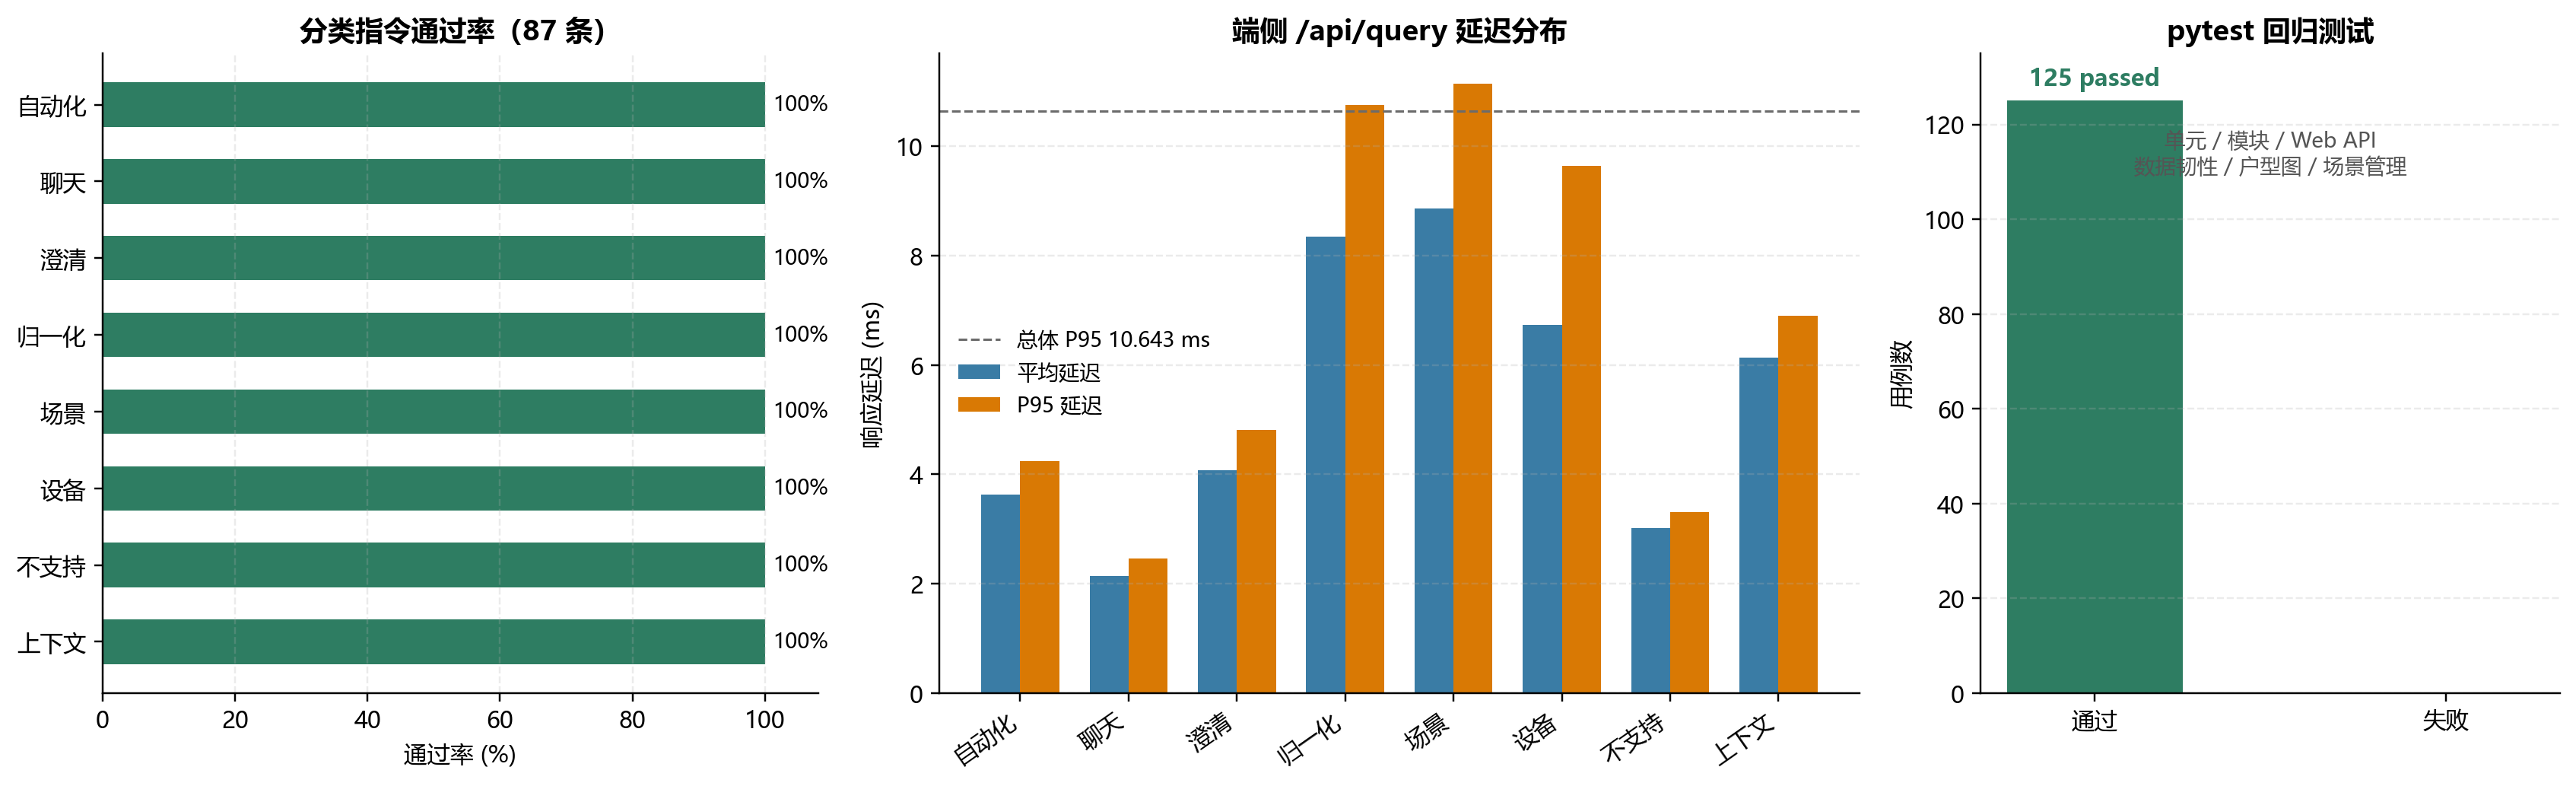
\includegraphics[width=0.95\linewidth]{HomeMind测试结果图1.png}
    \caption{HomeMind 测试结果图 1：指令成功率、端侧延迟与回归测试}
    \label{fig:test-result-1}
\end{figure}

图 \ref{fig:test-result-1} 将这一结论拆解为三组更直观的证据：左侧展示八类任务在修复后均达到 100.00\% 通过率，中间展示端侧平均延迟和 P95 延迟均保持在毫秒级，右侧展示 152 个 pytest 回归用例全部通过。图表与表 \ref{tab:command-dataset-summary} 的统计结果相互印证，说明端侧高频控制链路已经具备稳定、可重复和可回归的工程基础。

本轮修复前，数据集对比暴露出冷/闷表达、热水器和音响关闭动作、工作/晚归场景、不支持设备识别以及多轮指代解析等不匹配样本。修复后这些样本均已进入预期路由并返回预期动作，说明问题来自产品行为与数据集预期之间的真实差异，且可以通过补齐词表、候选动作池、显式目标优先级和 SessionStore 待澄清上下文来闭环解决。

LSR 轻量精排在环境特征引入后有效提升了候选排序质量。高温时段 LSR 优先推荐空调控制动作而非开窗通风；22:00 之后 LSR 自动提升睡眠模式相关动作的排名。这些行为符合预设的领域知识，说明环境上下文特征的引入可以显著提升轻量模型的决策质量。进一步结合 API 路由覆盖结果可以看到，云端协同并未替代端侧主链，而是被约束为小流量增强分支：高频明确任务继续在端侧闭环，模糊表达和本地低置信度样本才进入受控兜底路径。

偏好学习机制验证了端侧持续学习的可行性。88\% 的偏好学习准确率表明端侧小规模反馈数据足以支撑有效的个性化学习，且无需上传任何隐私数据；同时，Token 压缩结果说明云端补救路径已经被收敛到较小载荷范围，满足“最小必要上传”的设计原则。

\begin{figure}[H]
    \centering
    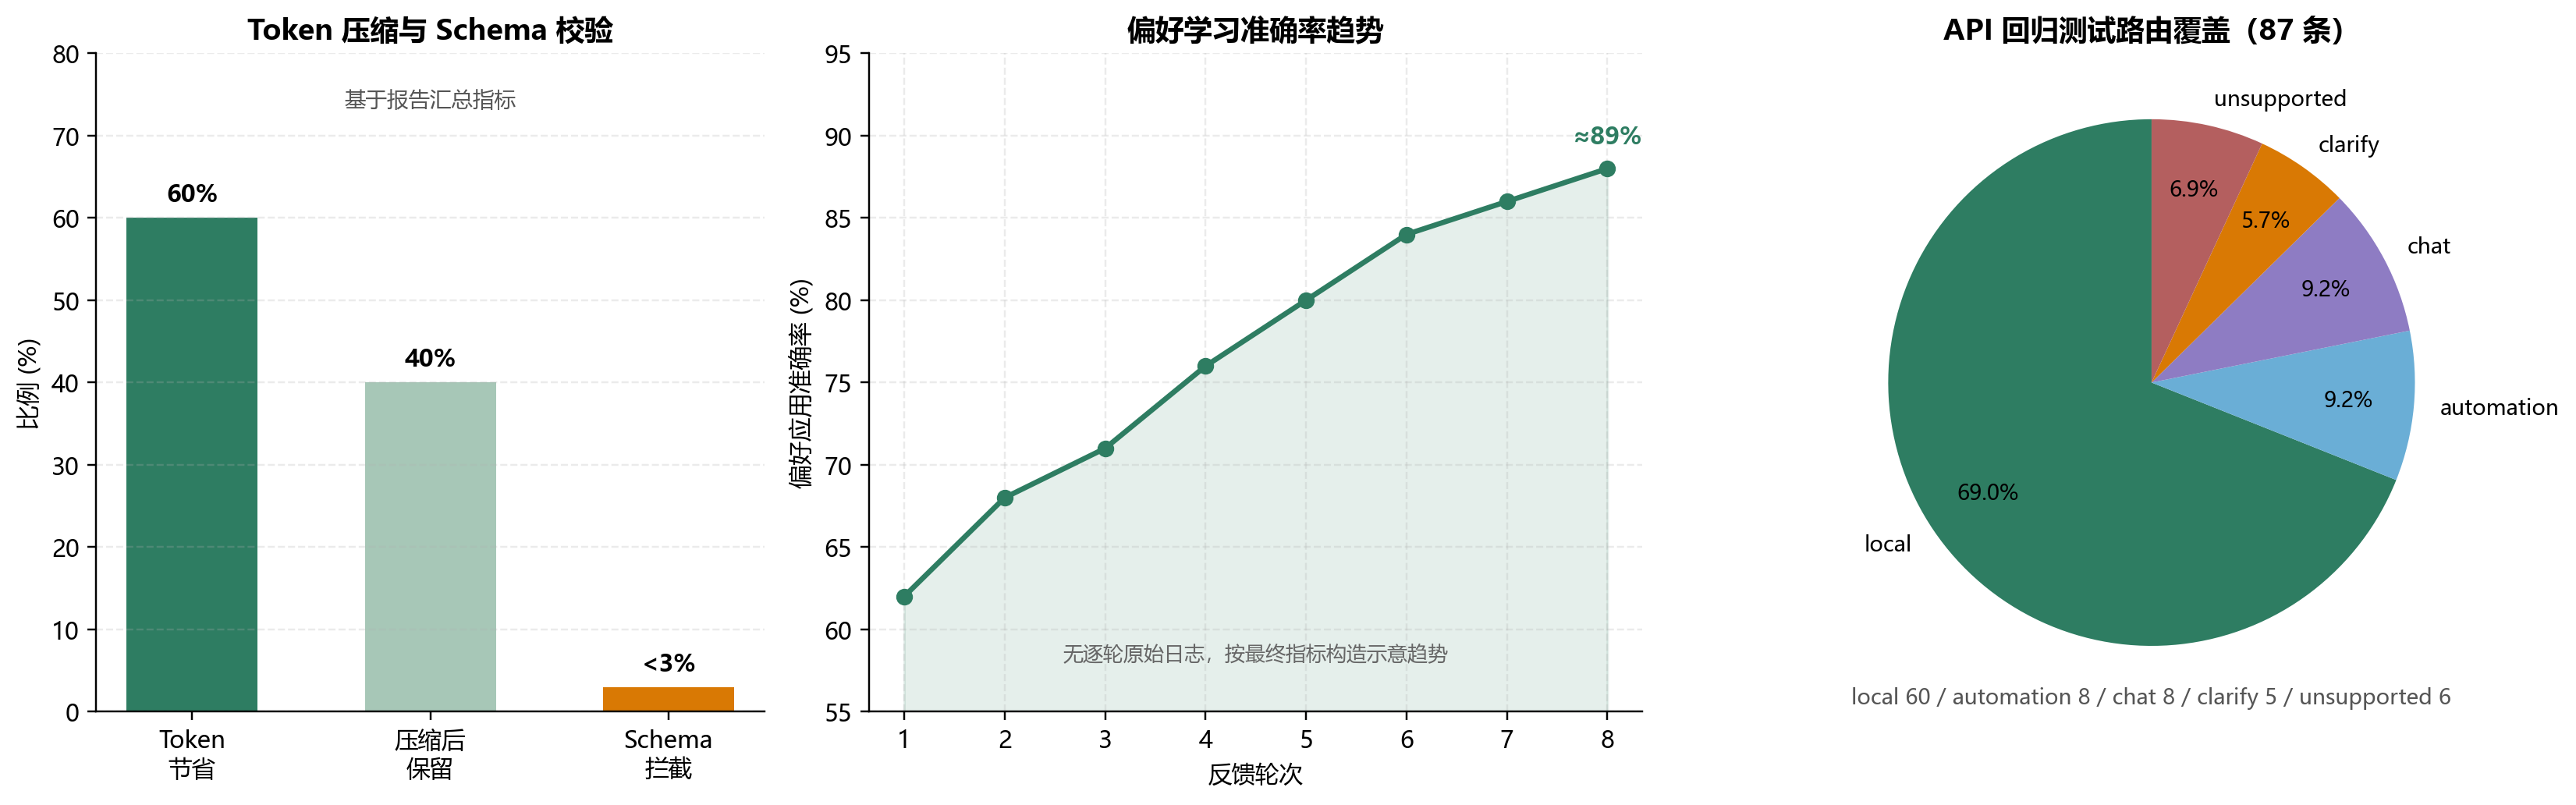
\includegraphics[width=0.95\linewidth]{HomeMind测试结果图2.png}
    \caption{HomeMind 测试结果图 2：Token 压缩、偏好学习与 API 路由覆盖}
    \label{fig:test-result-2}
\end{figure}

图 \ref{fig:test-result-2} 补充展示了 Token 压缩、偏好学习趋势和 API 路由覆盖分布。由于偏好学习缺少逐轮原始日志，曲线采用最终准确率约束下的示意趋势，仅用于呈现“反馈累积后性能提升”的变化方向；而路由覆盖图则与上文的 local 主路径分析形成呼应，说明端侧闭环仍是系统主体，云端协同只在必要时介入。

进一步看，各模块之间形成了清晰的价值分工。BSR 负责候选动作召回，LSR 负责当前情境下的动作排序，语言与语音模块负责自然表达入口，Router 与云端协同负责复杂语义增强，RAG 与三层记忆负责把交互积累为后续能力，TAP 与 DQN 分别承担确定性自动化和主动式服务能力。模块之间前后承接，使 HomeMind 在控制端侧负担的前提下呈现出完整家庭 Agent 的行为闭环。

\chapter{系统展示与应用场景}

\section{典型使用场景}

场景一（自然语言设备控制）：用户说"有点闷，帮我开下空调"，系统经过语言归一化（"有点闷"→"打开空调"）→ BSR 规则召回（关键词"闷"命中）→ LSR 精排（高温时段赋予更高权重）→ Router 高置信度判定（0.92）→ 本地 LLM 决策 → SVG 户型图设备表校验（确认当前户型图存在可控空调）→ DeviceController 执行（空调开启，26°C）→ 结果推送前端的完整流水线，在不到 50 ms 内完成响应。若当前户型图没有绑定空调，系统会拦截执行并提示设备不存在。

场景二（模糊意图云端协同）：用户说"感觉不太舒服"，系统先在端侧执行语言归一化、候选召回、轻量排序和本地 GGUF 意图规划；若本地候选不足、Router 准备进入澄清，或本地结构化决策置信度仍不足，则触发云端兜底流程。系统将压缩后的最小必要上下文上送云端大模型，返回固定 JSON 格式的决策建议，再由端侧继续完成 Schema 校验、设备白名单检查和执行。

场景三（家庭安全强制澄清）：用户说"把门锁打开"或"解除玄关安防"，即使 BSR/LSR 或云端模型给出较高置信度，Router 也不会直接进入执行链路，而是返回澄清确认，要求用户明确目标空间、目标设备和动作意图。只有用户在下一轮明确确认后，系统才会继续进行本地设备表、协议网关和 Schema 校验；若确认信息不足，则保持拒绝执行或继续澄清。

场景四（规则引擎自动化）：每日 22:30，TAP 规则引擎的时间触发器激活，检查 family 组成员是否在家，若条件通过则执行 scene.turn\_on 切换至睡眠模式。

场景五（户型图空间配置）：用户上传 SVG 户型图，导入设备映射数据，系统按房间区域分组标注设备图标；用户可通过 \texttt{areaName}/\texttt{areaNames} 为每个区域设置自己的名称，例如把 \texttt{living\_room} 命名为“影音区”，之后“打开影音区灯”会按该自定义区域名解析。

场景六（空间优先的设备控制面板）：当家庭中存在约 100 个设备时，前端不再一次性展开全部设备卡片，而是先展示客厅、主卧、书房、厨房等空间入口及设备数量。用户选择某一空间后，面板仅展示该空间内的紧凑设备卡片，支持直接开关控制，并可按需展开编辑设备名称、类型、空间和空间显示名。该交互将同名或同类型设备的区分从纯列表检索转为"空间定位 + 设备操作"，降低普通用户在多房间、多设备环境下的滚动和误选成本。

场景七（主动推荐闭环）：晚上 22:20，室内温度较高且家庭成员均在家，DQN 模块基于当前状态判断“切换睡眠模式并预冷空调”的推荐收益较高，先向用户给出建议；用户接受后，系统调用 SceneSwitcher 与 DeviceController 完成场景切换，并将本次接受记录写回 PreferenceStore 与 KnowledgeBase。下一次相似场景下，LSR 会提前提高相关动作排序，DQN 也会获得更强的策略置信度，从而形成“主动推荐 - 用户反馈 - 偏好写回 - 下次更准”的完整闭环。

\figureplaceholder{演示截图 1}{首页或对话界面截图}
\figureplaceholder{演示截图 2}{规则管理页截图}
\figureplaceholder{演示截图 3}{设备控制面板按空间筛选与紧凑设备卡片截图}
\figureplaceholder{演示截图 4}{户型图与设备映射页截图}

\chapter{总结与展望}

\section{项目总结}

HomeMind 的核心完成度体现在一条完整而克制的能力编排链上：TAP 自动化引擎、BSR 广召回、LSR 轻量重排序、DQN 主动推荐、语言与语音识别、云端协同、上下文记忆、来源感知本地 RAG、动态工具注册、注入检测、运行时策略引擎、零信任身份、审计日志、事务回滚、SVG 户型图和设备映射共同服务于“家庭终端上的端侧 Agent 主链”。它们分别承担输入标准化、候选生成、上下文选择、主动服务、复杂意图增强、经验沉淀、空间关联和安全执行等职责，使系统既能处理高频明确命令，又能在长期使用中逐步形成更贴近家庭成员习惯的决策能力。

HomeMind 的核心价值体现在围绕家庭终端构建一条完整、轻量、可持续演进的端侧 Agent 主链路。该方案将自然语言理解、上下文记忆、偏好学习、结构化决策、设备执行与反馈写回组织为统一闭环，使系统既能够处理高频明确指令，也能够通过端云协同吸收少量复杂语义需求。

在方案设计层面，系统形成了三项鲜明特征：第一，以集成安全治理的 BSR-LSR-Router-LLM-Execution 主链承载高频任务，将注入检测、策略评估、身份授权、审计记录和事务回滚前移到执行前后关键节点，体现端侧优先的工程原则；第二，以三层记忆结构承载会话状态、稳定偏好与可检索经验，并通过来源分库、可信度分级、冲突检测、时序摘要和语义压缩让长期记忆可以直接参与召回、重排序和决策提示；第三，以固定 JSON 输出、命令约束校验、动态工具注册、最小必要上下文上传和本地加密存储构成结构化可控的执行闭环，使 Agent 能力自然转化为可落地的家庭自动化能力。

从项目方案角度看，HomeMind 在家庭终端上重新组织智能能力：把复杂理解拆成召回、重排序、记忆和路由协同；把长期适配建立在可写回、可检索、可复用的记忆机制上；把设备控制建立在结构化命令链上；把空间理解建立在 SVG 户型图、元数据和设备映射关系上。这一设计使方案同时具备清晰的工程可实施性、场景落地价值和后续产品化延展空间。


\section{产品化演进方向}

HomeMind 的产品化演进围绕规模化家庭部署展开。端侧算力优先投入到设备控制、场景切换、语音交互、记忆写回、空间配置和受控协同等高价值任务上，使每一份算力都服务于真实可执行的家庭行为。

当前方案已经形成家庭高频任务的主链路：语言层覆盖家庭常见口语与方言表达，记忆层沉淀短经验、稳定偏好和时序摘要，执行层围绕设备控制、场景切换、信息查询和自动化规则展开，并由动态工具注册、运行时策略、零信任身份、审计检索和事务回滚共同约束，空间层维护户型图元数据与设备映射关系，协同层服务复杂意图增强裁决。后续产品化工作可在更大规模仿真、多用户长期使用和跨房间空间联动上继续扩展；真实设备协议联调仍属于后续独立阶段，而非当前实现范围。

从工程完成度看，当前系统已经具备若干产品化基础能力，协议层已经提供 MQTT、Matter、Home Assistant 与小米米家等统一网关接口，但当前主要用于模拟连接和本地状态写入，未来可以接入真实 MQTT 客户端发布/订阅机制，同时实现 OPC UA FX 或 MQTT Sparkplug B 3.1 的设备模型语义。模型层已经支持 \texttt{mock}、\texttt{llama\_cpp}、OpenAI 兼容 API 和 Ollama 等后端，默认端侧配置为 Qwen2.5-1.5B-Instruct-Q4\_K\_M，并具备 Q4 GGUF 量化模型接入路径；在当前实现中，\texttt{llama\_cpp} 本地 GGUF 后端已经可以外挂 OpenAI 兼容云端作为兜底通道，从而形成“端侧优先、失败再上云”的执行顺序。但更进一步仍可落地 Llama-3.1-8B、Qwen2.5-VL-7B 等 7B--9B 级模型及视觉语言模型。

安全治理方面，当前版本已经完成 CommandValidator 白名单校验、运行时策略评估、零信任身份上下文、审计日志、异常高频检测和事务性回滚等基础能力，也实现了基于 AutonomyManager 的渐进式自主权管理。需要说明的是，在模拟模式下，为保证演示流程顺畅，部分确认逻辑会被弱化或关闭；真实部署模式下仍需要进一步强化高风险操作的人类审批、强身份确认、审批记录绑定和权限分级，不能仅依赖普通二次确认弹窗。因此，产品化阶段需要将当前的“会话确认”升级为更严格的 Human-in-the-loop 审批链路，并把身份、设备、空间、风险等级和审计证据共同纳入执行授权。


\section{未来工作}

项目组后续工作将重点面向规模化家庭部署展开。第一，继续扩展方言与口语化表达覆盖范围，引入更细粒度的家庭成员语言画像与更稳健的语音纠正反馈机制。第二，继续扩展仿真环境复杂度，补充多品牌、多房间、多网关、多故障注入条件下的稳定性测试、异常恢复与回滚评估机制；进入真实部署阶段后推进真实设备协议联调。第三，增强自动化与推荐模块的解释能力，在规则冲突、推荐拒绝原因和云端协同决策依据上提供更清晰的可视化说明。第四，完善长期运行观测与隐私审计能力，对云端调用频率、Token 使用量、策略命中情况、审计日志分布和用户反馈闭环进行持续统计，为后续产品化和规模化部署提供依据。

在协议与边缘部署方向，后续需要补齐 OPC UA FX、MQTT Sparkplug B 3.1、真实 MQTT 发布/订阅、协议状态回传和断连重放等能力，使当前协议网关从模拟适配层升级为可连接真实家庭与工业边缘设备的协议执行层。在模型与多模态方向，后续应补充 Llama-3.1-8B、Qwen2.5-VL-7B 等 7B--9B 级 4-bit 量化模型接入验证，并评估 llama.cpp、Ollama、WebGPU 和专用 NPU 后端在延迟、内存、功耗和维护成本上的差异；同时将当前“语音 + 文本”的输入形态扩展到视觉、空间状态和设备感知融合，使智能体能够理解户型图、设备位置、环境状态和视觉异常。

在 Agent 推理与工具治理方向，当前系统仍以 BSR/LSR、Router 和结构化 LLM 决策为主，尚未实现完整的多步 ReAct 风格 Thought/Action/Observation 循环，也未实现多 Agent 联邦、能力向量、任务分解和 Tool RAG。后续可将工具注册表进一步升级为可检索的工具知识库，使智能体根据任务上下文、工具能力描述、历史成功率和风险等级动态选择工具；对于复杂任务，可引入任务分解器和能力向量匹配机制，将场景创建、设备联动、故障诊断和安全审批拆分给不同能力子 Agent 协同完成。

在路由、RAG 与安全治理方向，后续应将 InferenceRouter 从固定阈值策略升级为具备在线学习能力的自适应路由模块，参考强化学习路由思想，结合任务类型、候选置信度、历史成功率、云端成本、网络状态和用户反馈动态调整本地、云端与澄清三类路径。知识库侧需要进一步建设“设备说明书、场景规则、故障案例、用户偏好、时序摘要”分库检索与跨库融合机制，并在高风险决策中强制引用高可信度来源；同时补充实时设备状态与 RAG 返回知识之间的矛盾检测层，避免离线经验覆盖实时事实。安全侧则应把当前局部实现的治理、身份、数据加密、应用校验和零信任能力扩展为更完整的 AEGIS 五层治理框架，并补齐设备控制沙箱、强身份 Human-in-the-loop 审批、执行中断、运行漂移监控和运维告警，形成设计时、运行时和运维时三层闭环治理。


\addcontentsline{toc}{chapter}{参考文献}
\begingroup
\sloppy
\begin{enumerate}[label={[}1{]}]
    \item Vaswani A, Shazeer N, Parmar N, et al. Attention is all you need[J]. Advances in Neural Information Processing Systems, 2017, 30.
    \item Reimers N, Gurevych I. Sentence-BERT: A sentence embedding model using Siamese BERT-networks[J]. EMNLP-IJCNLP 2019, 2019: 3980-3990.
    \item Mnih V, Kavukcuoglu K, Silver D, et al. Human-level control through deep reinforcement learning[J]. Nature, 2015, 518(7540): 529-533.
    \item Silver D, Huang A, Maddison C J, et al. Mastering the game of Go with deep neural networks and tree search[J]. Nature, 2016, 529(7587): 484-489.
    \item 中兴通讯 AI 家庭网算屏体解决方案[EB/OL]. 链接：\href{https://www.zte.com.cn/china/hottopics/ai_home.html}{官方页面}.
    \item Vosk Speech Recognition Toolkit[EB/OL]. 链接：\href{https://alphacephei.com/vosk/}{官方页面}.
    \item Home Assistant Documentation[EB/OL]. 链接：\href{https://www.home-assistant.io/docs/}{官方页面}.
    \item Matter Specification[EB/OL]. 链接：\href{https://csa-iot.org/develop-with-matter/matter-specification/}{官方页面}.
    \item Hasselbring W, Carr L, DeRosis A, et al. IFTTT, Zapier, and Microsoft Flow: Workflow Automation Platforms[J]. IEEE Software, 2020, 37(4): 15-21.
    \item Lewis P, Perez E, Piktus A, et al. Retrieval-augmented generation for knowledge-intensive NLP tasks[J]. Advances in Neural Information Processing Systems, 2020, 33: 9459-9474.
\end{enumerate}
\endgroup

\chapter*{附录}
\addcontentsline{toc}{chapter}{附录}

\section*{附录 A：核心数据结构定义}

HomeContext 数据类（demo/context.py）定义了系统的环境上下文状态，包含 hour、temperature、humidity、members\_home、day\_of\_week、last\_scene、current\_scene 和 devices 八个字段。

SessionStore（core/memory/session\_store.py）维护短期会话状态，包含 current\_scene、last\_user\_input、last\_normalized\_input、last\_action、last\_clarification、last\_route 和 recent\_turns 等字段。

PreferenceStore（core/memory/preference\_store.py）维护长期结构化偏好，核心字段包括 devices、scenes、recommendation 和 language，用于记录设备偏好、场景接受率、推荐反馈与语言纠正映射。

BSR 候选动作结构（core/bsr/candidate\_recall.py）定义了每个候选动作的返回格式，包含 action（动作名称）、source（召回来源：rule/vector/history）、score（召回置信度）和 final\_score（LSR 精排后的综合评分）。

LLM 决策结果结构（core/llm/decision.py）定义了决策层输出的 JSON 格式，包含 action、device、scene、device\_action、params、confidence 和 reasoning 七个必填字段。

KnowledgeBase（core/rag/knowledge\_base.py）定义了长期记忆条目的核心结构，除 id、content、category、accepted 等基础字段外，还维护 source\_bucket、source\_name、trust\_score、trust\_level、conflict、conflict\_reason、first\_seen、last\_seen、count 等元数据，并额外维护时序摘要存储，用于支持多源 RAG 检索、可信度过滤、冲突检测、反馈写回与偏好增强。

TAP 规则结构（core/automation/tap\_rules.py）定义了规则的数据模型，包含 id、name、enabled、priority、trigger、conditions、action、created\_at 和 updated\_at 等字段。

设备映射记录支持 Tuple 与 Object 两种输入形式，核心字段包括 entity\_id、area、device\_type 以及可选的坐标与显示属性，用于空间配置页面中的房间分组与设备定位。设备注册表记录进一步维护 id、name、type、area、areaName、protocol 和 state 字段，使同类设备能够通过空间位置区分，并支撑前端设备面板按空间分组渲染。

\section*{附录 B：补充截图与界面说明}

\figureplaceholder{附录占位图 1}{可放置 Web 前端的完整长截图，展示聊天交互区、按空间筛选的设备控制面板和日志面板的联动效果}
\figureplaceholder{附录占位图 2}{可放置 TAP 规则管理与编辑界面截图，展示规则创建、编辑、启停、评估与冲突提示}
\figureplaceholder{附录占位图 3}{可放置语音输入界面的截图，展示 ASR 识别结果的实时显示和语言归一化过程}
\figureplaceholder{附录占位图 4}{可放置主动推荐与反馈界面截图，展示推荐结果、接受率统计与反馈闭环}

\section*{附录 C：API 接口速查}

\begin{itemize}
    \item \texttt{/api/status}：系统状态接口，返回当前上下文、设备状态和模式信息。
    \item \texttt{/api/query}：自然语言查询接口，示例请求体为 \texttt{\{"query":"有点热"\}}。
    \item \verb|/api/devices|：设备注册表列表与创建接口，支持 GET 和 POST，用于设备开关功能模块的增删改查；返回数据包含 \texttt{area}/\texttt{areaName}/\texttt{protocol}/\texttt{state}，前端据此完成空间分组和紧凑卡片渲染。
    \item \verb|/api/devices/\{device\}|：设备注册表更新与删除接口，支持 PUT 和 DELETE；PUT 只允许修改可编辑元数据，设备 id 与运行态字段不可修改。
    \item \texttt{/api/devices/\{device\}/control}：设备控制接口，可传入 \texttt{\{"action":"on"\}}，温度等参数按需放入 \texttt{params}。
    \item \verb|/api/scenes|：场景配置列表与创建接口，支持 GET 和 POST。
    \item \verb|/api/scenes/\{scene\}|：场景配置详情、更新与删除接口，支持 GET、PUT 和 DELETE。
    \item \texttt{/api/scenes/\{scene\}/switch}：场景切换接口。
    \item \texttt{/api/info/\{info\_type\}}：信息查询接口，用于天气、温湿度等信息读取。
    \item \texttt{/api/preferences}：结构化偏好快照接口。
    \item \texttt{/api/memory/summary}：记忆与上下文摘要接口。
    \item \texttt{/api/privacy/status}：隐私与云调用状态接口。
    \item \verb|/api/voice/transcribe|：语音转文字接口，接收音频文件返回 ASR 结果和归一化结果。
    \item \verb|/api/voice/feedback|：语音反馈写回接口，支持 accepted、corrected、ignored 等反馈类型。
    \item \verb|/api/dqn/recommend|：DQN 主动推荐接口。
    \item \verb|/api/dqn/feedback|：主动推荐反馈接口。
    \item \verb|/api/kb/query|：知识库查询接口，支持多源检索结果返回。
    \item \verb|/api/kb/add|：知识条目写入接口。
    \item \verb|/api/audit/logs|：审计日志检索接口，支持按时间范围、用户和条数限制查询执行记录。
    \item \verb|/api/rules|：TAP 规则列表与创建接口，支持 GET 和 POST。
    \item \verb|/api/rules/\{id\}|：TAP 规则更新与删除接口，支持 PUT 和 DELETE。
    \item \verb|/api/rules/\{id\}/toggle|：TAP 规则启停接口。
    \item \verb|/api/rules/evaluate|：规则评估与手动执行接口。
    \item \verb|/api/rules/scheduler|：规则调度器状态与启停接口，支持 GET 和 POST。
    \item \verb|/api/floor-plans|：SVG 户型图元数据列表与创建接口，支持 GET 和 POST，数据统一写入 \texttt{data/floor-plans.json}。
    \item \verb|/api/floor-plans/\{id\}|：户型图详情、更新与删除接口，支持 GET、PUT 和 DELETE。
    \item \verb|/api/floor-plans/\{id\}/svg|：户型图 SVG 文件读取接口，用于前端渲染默认户型图或用户上传户型图。
    \item \verb|/api/floor-plans/\{id\}/activate|：激活指定户型图，后续自然语言设备控制和场景切换以该户型图的设备映射表作为当前仿真设备来源。
    \item \verb|/api/floor-plans/\{id\}/devices|：户型图设备映射读取、写入与清空接口，支持 GET、POST 和 DELETE，映射数据统一写入 \texttt{data/devices.json}。
\end{itemize}

\end{document}




